\documentclass[a4paper,11pt,twoside]{book}

\usepackage{my-thesis-template}


%----------------------------------------------------------------------------------------
%	METADATA
%----------------------------------------------------------------------------------------
\newcommand{\thesistitle}{Robotic surgical tool manipulator - Recognition, control and manipulation of laparoscopic tools}
\newcommand{\division}{Division}
\newcommand{\me}{Karadimos Alexios of Loukas}
\newcommand{\nomme}{Karadimos Alexios of Loukas}
\newcommand{\studnum}{1046820}
\newcommand{\monthyear}{Month 2021}
\newcommand{\supname}{Evangelos Dermatas}
\newcommand{\suptitle}{Associate Professor Dr.}
\newcommand{\cosupname}{Anthony Tzes}
\newcommand{\cosuptitle}{Professor Dr.}
\newcommand{\headofdivision}{Kazakos Demosthenes}
\newcommand{\headofdivisiontitle}{Assistant Professor Dr.}
\newcommand{\keywords}{surgery, robotics, control, laparoscopy, RCM, fulcrum, MIS, trajectory, ROS}
\title{\thesistitle}
\author{Karadimos Alexios}
\date{2020}

% PDF metadata
\hypersetup
{
    pdfauthor={Alexios Karadimos},
    pdftitle={thesis},
    pdfsubject={\thesistitle},
    pdfkeywords={\keywords},
    pdfproducer={PdfLaTex},
    pdfcreator={Alexios Karadimos}
}


\begin{document}

\selectlanguage{greek}
\selectlanguage{english}


%----------------------------------------------------------------------------------------
%	FRONT PAGE & CERTIFICATION
%----------------------------------------------------------------------------------------
\begin{titlepage}
\begin{center}
% Upper part of the page
\textsc{\textbf{\large UNIVERSITY OF PATRAS - SCHOOL OF ENGINEERING}\\
\large DEPARTMENT OF ELECTRICAL AND COMPUTER ENGINEERING}\\

\includegraphics[width= 0.5\textwidth]{up_2017_logo_gr.png}\\  

\textsc{Division: \large Systems and Automatic Control}\\[1cm]

\textsc{\textbf{\LARGE{Thesis}}}\\ [0.5cm]
of the student of the Department of Electrical and Computer Engineering of the School of Engineering of the University of Patras\\[0.5cm]

\textsc{\Large \me }\\[0.5cm]
\textsc{\large Student Number: 1046820}\\[1cm]

\underline{\large Subject}\\
\HRule \\[0.4cm]
{\huge \bfseries \thesistitle }\\[0.4cm] % Title of your document
\HRule \\[1.5cm]

\underline{\large Supervisor}\\[0.5cm]
\large \suptitle \, \supname \\[1cm]
\textbf{Thesis Number:}
%\large 1046820/2020
\vfill
% Bottom of the page
\large{Patras, 2020}
\end{center}
\end{titlepage}

% \begin{titlepage}

% %----------------------------------------------------------------------------------------
% %	HEADING SECTIONS
% %----------------------------------------------------------------------------------------

% \Large UNIVERSITY OF PATRAS - SCHOOL OF ENGINEERING\\[0.5cm] % Name of your university/college
% \textsc{\Large DEPARTMENT OF ELECTRICAL AND COMPUTER ENGINEERING}\\[0.5cm] % Major heading such as course name
% \textsc{\large \textlatin{ECE}ΔΚ803}\\[0.5cm] % Minor heading such as course title

% %----------------------------------------------------------------------------------------
% %	TITLE SECTION
% %----------------------------------------------------------------------------------------


% %----------------------------------------------------------------------------------------
% %	AUTHOR SECTION
% %----------------------------------------------------------------------------------------


% % If you don't want a supervisor, uncomment the two lines below and remove the section above
% %\Large \emph{Author:}\\
% \emph{Αλέξιος Καραδήμος}\\ % Your name
% Τμήμα Ηλεκτρολόγων Μηχανικών \& Τεχνολογίας Υπολογιστών\\[2cm]

% %----------------------------------------------------------------------------------------
% %	DATE SECTION
% %----------------------------------------------------------------------------------------

% {\large 2020}\\[1cm] % Date, change the \today to a set date if you want to be precise

% %----------------------------------------------------------------------------------------
% %	LOGO SECTION
% %----------------------------------------------------------------------------------------

% \begin{center}
% \includegraphics[width=5cm]{images/up_2017_logo_gr.png}\\[1cm] % Include a department/university logo - this will require the graphicx package
% \end{center}

% %----------------------------------------------------------------------------------------

% \vfill % Fill the rest of the page with whitespace

% \end{titlepage}

\pagestyle{empty}
\begin{center}
{\LARGE \textbf{CERTIFICATION}\\[1cm]}
\large It is certified that the Diploma Thesis titled\\[1cm]
\textbf{\large \thesistitle }\\[1cm]
of the Department of Electrical and Computer Engineering student\\[1.5cm]
\textbf{\large \me }\\[0.5cm]
Registration Number: \studnum \\[1.5cm]
was presented publicly at the Department of Electrical and Computer Engineering at\\[0.5cm]
\Large{02/02/2022}\\[0.5cm]
and was examined by the following examining committee:\\[0.5cm]
\supname, \suptitle (supervisor)\\
Konstantinos Moustakas, Professor (committee member)\\
Kyriakos Sgarbas, Associate Professor (committee member)\\
\end{center}

\vfill

\begin{minipage}{0.5\textwidth}
\begin{flushleft} \large
The supervisor\\[3cm]
\supname \\
\emph{\suptitle}
\end{flushleft}
\end{minipage}
\begin{minipage}{0.5\textwidth}
\begin{flushright} \large
The Director of the Division\\[3cm]
\headofdivision\\
\emph{\headofdivisiontitle}
\end{flushright}
\end{minipage}

\pagestyle{empty}
\begin{center}

{\large \textbf{Thesis details}\\[1cm]}

\textbf{\large \thesistitle }\\[1cm]

\pagestyle{empty}
{\textbf{Abstract}\\[1cm]}

This thesis studies all the stages involved in the recognition, control and manipulation of laparoscopic tools in an end-to-end approach with more emphasis given to the pivot trajectories and the RCM constrained motion 
planning. The first step was to study the forward and inverse kinematics of the KUKA iiwa14 industrial robot arm (with the position-orientation decoupling technique for 6dof robots, leaving the extra degree of freedom to be 
specified by other constraints) as well as kinematics of the Barrett hand gripper in order to calculate grasps. Since MIS robotics is very constrained in nature, the next step was to study the RCM constraint for the pivot 
motions, the elbow-up constraint to avoid collisions as well as the workspace constraints and singularities. When designing robot applications it is important to study the robot’s workspace, and for this reason, this thesis 
also studies the surgical task space and how this is transformed to the robot’s taskspace and the joint space. The manipulability of the robot was also studied and also a suitable environment layout so that all trajectories 
were well reachable. A lot of emphasis was given in calculating various geometric paths for the robot to follow inside the surgical task. The equations for circular, circular arc, line segment, helical, cubic spline, b-spline, 
higher-order polynomial and trapezoid and s-curve velocity profile trajectories are studied in detail in order to generate pivot motions with a wide variety. All experiments were conducted using the ROS framework and popular 
tools and libraries like Gazebo, RViz and MoveIt using the RRTConnect path planning algorithm. The experiments were evaluated with measurements of time, position accuracy and RCM distance deviation. This thesis also briefly 
studies a simple recognition of a laparoscopic tool and the estimation of it’s position and orientation using computer vision as well as the calculation of 3 points on the surgical tool where the gripper’s fingers will be 
placed in order to grasp the object with a satisfactory force closure. Finally this thesis studies some control system schemes like for example the RCM tracking and pivot motion control.

\newpage{\pagestyle{empty}\cleardoublepage}

\newpage
\pagestyle{empty}
{\textbf{Περίληψη}\\[1cm]}

Η παρούσα διπλωματική εξετάζει όλα τα στάδια που εμπλέκονται στην αναγνώριση, τον έλεγχο και τον χειρισμό των λαπαροσκοπικών εργαλείων με μια ολιστική προσέγγιση αλλά με μεγαλύτερη έμφαση να δίνεται στις τροχιές περιστροφής 
γύρω από σημείο και στον προγραμματισμό περιορισμένης κίνησης RCM. Το πρώτο βήμα ήταν να μελετηθεί το ευθύ και αντίστροφο κινηματικό πρόβλημα του βιομηχανικού ρομποτικού βραχίονα KUKA iiwa14 (με την τεχνική αποσύνδεσης θέσης-
προσανατολισμού για ρομπότ 6 βαθμών ελευθερίας, αφήνοντας τον επιπλέον βαθμό ελευθερίας να καθοριστεί από άλλους περιορισμούς) καθώς και η κινηματική της αρπάγης Barrett ώστε να υπολογιστούν λαβές του χειρουργικού εργαλείου. 
Δεδομένου ότι η ρομποτική MIS επιβάλλει πολλούς περιορισμούς, το επόμενο βήμα ήταν να μελετηθεί ο περιορισμός RCM για τις κινήσεις περιστροφής (pivot), o περιορισμός στον οποίο ο αγκώνας του ρομπότ πρέπει να είναι προς τα πάνω 
για την αποφυγή συγκρούσεων καθώς και οι περιορισμοί και τα σημεία ενικότητας του χώρου εργασίας. Κατά το σχεδιασμό εφαρμογών ρομπότ είναι σημαντικό να μελετηθεί ο χώρος εργασίας του ρομπότ και για το λόγο αυτό, αυτή στη 
διπλωματική αυτή μελετάται επιπλέον ο χώρος χειρουργικών εργασιών και πώς αυτός μετατρέπεται στον χώρο εργασιών του ρομπότ και στον χώρο αρθρώσεών του. Μελετήθηκε επίσης ο δείκτης επιδεξιότητας του ρομπότ και η κατάλληλη 
διάταξη του ρομπότ σε σχεση με το περιβάλλον του έτσι ώστε όλες οι τροχιές να είναι καλά προσβάσιμες και να μπορουν να εκτελεστούν με ευκολία. Δόθηκε μεγάλη έμφαση στον υπολογισμό διαφόρων γεωμετρικών μονοπατιών που έπρεπε να 
ακολουθήσει το ρομπότ μέσα στο χώρο χειρουργικής εργασίας. Οι εξισώσεις για τροχιές κύκλου, κυκλικού τόξου, ευθύγραμμου τμήματος, έλικα, κυβικού spline, b-spline, πολυωνύμων υψηλότερης τάξης και τροχιές με προφίλ ταχύτητας 
τραπεζοειδές και καμπύλης-s, μελετώνται λεπτομερώς, προκειμένου να δημιουργηθούν χειρουργικές ρομποτικές κινήσεις με μεγάλη ποικιλία. Όλα τα πειράματα υλοποιήθηκαν χρησιμοποιώντας το περιβάλλον ROS και δημοφιλή εργαλεία και 
βιβλιοθήκες όπως τα Gazebo, RViz και MoveIt χρησιμοποιώντας τον αλγόριθμο σχεδιασμού διαδρομής RRTConnect. Τα πειράματα αξιολογήθηκαν με μετρήσεις χρόνου, ακρίβειας θέσης και απόκλισης απόστασης RCM. Στη διπλωματική αυτή 
μελετάται επίσης εν συντομία η απλή αναγνώριση ενός λαπαροσκοπικού εργαλείου και η εκτίμηση της θέσης και του προσανατολισμού του με χρήση υπολογιστικής όρασης καθώς και ο υπολογισμός 3 σημείων πάνω στο χειρουργικό εργαλείο 
όπου θα τοποθετηθούν τα δάχτυλα της αρπάγης για να πιάσει το αντικείμενο με μία ικανοποιητική λαβή. Τέλος, σε αυτή τη διπλωματική μελετώνται ορισμένα συστήματα ελέγχου όπως για παράδειγμα ενός συστήματος για την παρακολούθηση 
RCM και τον έλεγχο κίνησης περιστροφής.


\pagestyle{empty}
{\textbf{Αcknowledgements}\\[1cm]}

The subject of this thesis, is a subject that I have been passionate about for many years and from the beginning of my university studies. For this reason 
I would like to thank my supervisors for giving me the opportunity to dive deep into this fascinating subject. I would also like to thank my friends and 
family for their huge support and for pushing me during the pandemic to conquer my academic goals.



%----------------------------------------------------------------------------------------
%	TABLE OF CONTENTS
%----------------------------------------------------------------------------------------

\pagestyle{fancy}

\clearpage
\tableofcontents
\renewcommand*\contentsname{Table of Contents}

%----------------------------------------------------------------------------------------
%	MAIN SECTIONS
%----------------------------------------------------------------------------------------

\newpage
\chapter{Introduction}

\section{Surgical robotics}

\subsection{Historical Overview of Surgical robotics}

Surgical robotics is a field of Surgery where the surgeon operaties on the patient via a computer, specialised equipment and robotic arms, 
to which the surgical tools needed for the operation are attached. According to surgical bibliography, robotics and laparoscopic procedures are used 
in general surgery, cardiothoracic surgeries, colon surgeries, gynecology, neurosurgery and orthopedics. \\

Robotic mechanisms were first introduced in Medicine, in 1987 with the first laparoscopic surgery of a cholecystectomy. Since then numerous laparoscopic 
operations have been performed and there has been a lot of improvements and innovations in this field. Such surgical operations are characterised as 
\textbf{minimally invasive}, because the surgical incisions made at the patient are very small and thus the probability of infection of the patient during 
or after the operation are very small, the hospitalization time is reduced (which means mean better and more efficient use of hospital resources) and the overall 
recovery of the patient is significantly faster and less painful. \\

However, traditional laparoscopic mechanisms have some downsides as well. First of all, the surgeon should operate in a mirrored-way, meaning that they should 
move at the opposite direction from what they saw at the screen (this effect is also known as the \textbf{fulcrum effect}), in order to reach the desired point of operation. Earlier laparoscopic tools had less 
degrees of freedom, which means less flexibility in motion control. Moreover these systems provided limited touch sensibility and feedback to the doctor they 
were very susceptible to the surgeon's micro movements and tremble. \\

The first application of robotics in Surgery appears in 1985, when Kwoh et al. \cite{Shao1985ANC} used a \textbf{PUMA 560}, a standard industrial robotic arm, to perform a neurosurgical biopsy, 
where the biopsy needle was inserted in the brain and guided with the help of Computed Tomography. This successful application was followed by the \textbf{PROBOT} surgical robot \cite{Probot1992}, 
which was developed at the Imperial College and used in a prostatectomy operation. Another example of an early surgery robot was the \textbf{ROBODOC} system \cite{Robodoc} developed by Integrated Surgical Supplies 
in Sacramento California, which was the first to be used in orthopedics for a hip replacement surgery and was also the first to be approved by the FDA (Food \& Drug Administration, organization responsible 
for medical devices, drugs etc.).

\begin{center}
\begin{figure}[!htb]
\centering
\includegraphics{images/Puma560.jpg}\\
\caption{The PUMA 560 robotic arm, which was the first to be used in surgery robotics in 1985}
\end{figure}
\end{center}

Some other important surgery robots are listed below:
\begin{itemize}
\item \textbf{AESOP\textsuperscript \textregistered Endoscope Positioner}: A voice controlled endoscopic system
\item \textbf{HERMES\textsuperscript \textregistered Control Center}
\item \textbf{daVinci Surgical System\textsuperscript \textregistered}: One of the most popular surgery robots and most used 
in hospitals. It is a master-slave system, which means that the operation commands are sent uni-directionally from the master 
console, which is controlled by the surgeon, and are executed by the robot. It also comes with a high definition 3D video feed 
and advanced manipulator system, one for each hand, called EndoWrist\textsuperscript \textregistered. It is officially approved 
by the FDA for laparoscopic surgeries.
\item \textbf{SOCRATES Robotic Telecollaboration System}
\item \textbf{Raven-II} \cite{Raven2}: An open platform for collaborative research on surgical robotics.
\item \textbf{Monarch\textsuperscript \texttrademark Platform} by Auris Health Inc., an endoscopic system for robotic-assisted 
bronchoscopy
\end{itemize}

\begin{center}
\begin{figure}[!htb]
\centering
\includegraphics[width=0.7\textwidth]{images/intuitive-da-vinci-xi-patient-cart-front-view-1060867-lo-res.jpg}\\
\caption{DaVinci Xi, \textsuperscript \textcopyright 2020 Intuitive Surgical, Inc. Patient Cart with the robotic arms that control the surgical tools}
\end{figure}
\end{center}

\begin{center}
\begin{figure}[!htb]
\centering
\includegraphics[width=0.8\textwidth]{images/Moarch_Platform_1200_x_676_1_.jpg}\\
\caption[The Monarch\textsuperscript \texttrademark Platform endoscopic system]{The Monarch\textsuperscript \texttrademark Platform endoscopic system \footnotemark}
\end{figure}
\end{center}
% How to use caption with footnote https://tex.stackexchange.com/questions/10181/using-footnote-in-a-figures-caption 
\footnotetext{\url{https://www.aurishealth.com/patients/robotic-bronchoscopy-patient-about-monarch-platform }}


\subsection{Surgical Robotics Procedure}

The robotic surgery procedure starts with total anesthesia of the patient. Then the surgeon makes small incisions at the anatomical region of interest, where the procedure will take place. Through 
these small incisions special tubes, called trocars, are mounted, through which the laparoscopic tools are inserted. After the patient is prepared and after the patient cart, which carries the robotic arms, 
is successfully positioned and callibrated, the surgeon sits on a console, from where they control they robot via special sensitive joysticks. The surgeon has vision access (often in 3D) to the surgical site via a
small endoscopic camera and the video is displayed on the console. In some cases, the surgeon gets force feedback from the joysticks via haptic mechanisms. Haptic force feedback is very important for the doctor 
in order to have a better sense of the anatomy and the surgical site, and it has gained a lot of interest in the reasearch community.

\begin{center}
\begin{figure}[!htb]
\centering
\includegraphics[width=0.5\textwidth]{images/intuitive-davinci-console-front-lowres.jpg}\\
\caption[DaVinci Xi \textsuperscript \textcopyright 2020 Intuitive Surgical, Inc. Surgeon Console]{DaVinci Xi \textsuperscript \textcopyright 2020 Intuitive Surgical, Inc. Surgeon Console \footnotemark}
\end{figure}
\end{center}
\footnotetext{\url{https://www.intuitive.com/en-us/about-us/press/press-resources}}


\subsection{Advantages \& Disadvantages of Surgical robotics}

Surgical robotics have a huge impact in Medicine and Healthcare in general. Some of the advantages are the following:
\begin{itemize}
\item \textbf{Minimally Invasive Procedures} which means
	\begin{itemize}
	\item Smaller incisions
	\item Less blood loss
	\item Reduced risk of inpatient infection
	\item Less pain
	\item Faster patient recovery
	\end{itemize}
\item Increased \textbf{precision} and reduced human errors
	\begin{itemize}
	\item Smooth and precise movements
	\item Detection and correction of errors caused by hand tremble
	\end{itemize}
\item \textbf{No fulcrum effect} and intuitive manipulation of surgical tools
\item \textbf{Haptic feedback}. This technology uses small mechanical forces and vibrations to give the user the sense of touch or force. Force feedback gives the ability to the surgeon to understand the 
mechanical properties of the tissue they operate on, such as resistance and elasticity, and thus distinguish between healthy from unhealthy tissue
\item \textbf{Teleoperation} (currently in the same room only): the surgeon operates while they sit on a special \textbf{ergonomic} console, which makes 
the long procedures more comfortable and efficient.
\end{itemize} 

\section{Problem statement}

The goal of this thesis is to design the kinematic models and algorithms necessary for a robotic arm to detect, pick and manipulate a laparoscopic surgical tool. To achieve these goals the robotic arm must 
successfully do the following:
\begin{itemize}
\item Use computer vision to detect the scene and laparoscopic tools and with the help of stereoscopic vision, calculate the position and orientation of the center of mass of each tool, with respect to the 
universal reference frame
\item Calculate the contact points on the tool, on which the fingers of the gripper will be placed, so that there is a firm grasp (force closure)
\item Calculate the path from the tools' table to the surgical site table
\item Calculate the trajectory that needs to be executed when the tool is inserted in the trocar. This is a special type of trajectory, because the motion is constrained and is known in the bibliography as
a \textbf{Remote Center of Motion} (RCM) control. The constraint is that, at each time one point of the inserted tool must coincide with the RCM point (this point will also be referenced in this thesis as the center of the 
trocar, or the fulcrum reference frame point).
\end{itemize}

\section{Bibliography Overview}

\section{Methodology \& Approach}

Robotics and especially surgery robotics is a multi-disciplinary field and a robot has many subsystems. A very important approach to successfully design a robotic arm to execute a surgery task is to subdivide the 
task in multiple smaller submodules and design, implement and test each submodule separately and then combine them together for end-to-end testing.

\begin{center}
\begin{figure}[!htb]
\centering

\includegraphics[width=0.15\textwidth]{images/motion-planning.png}\\
\caption{Motion planning pipeline}
\end{figure}
\end{center}

\textbf{Tools \& Software used in this thesis}:
\begin{itemize}
\item Matlab \& Matlab toolboxes: ROS Toolbox, Robotics Toolbox
\item ROS Framework
\item MoveIt
\item Gazebo simulator
\item VREP simulator
\item OpenCV
\end{itemize}

\textbf{Methodology of conducting this thesis}:
\begin{itemize}
\item Mathematical calculations for Kinematics and Motion planning
\item Mathematics validation with Matlab
\item Quick prototyping and testing with Matlab and/or VREP
\item Implementation in ROS frameworks, by splitting the end-to-end robotic operation in smaller 
experiments and tasks
\end{itemize}

\begin{center}
\begin{figure}[!htb]
\centering
\includegraphics[width=0.7\textwidth]{images/task-backlog-airtable.png}\\
\caption{Kanban view of backlog tasks to organize all features, requirerements and tasks needed to complete this thesis. The tool used to keep track of all tasks is Airtable}
\end{figure}
\end{center}

To quickly test out ideas on how to build the robot's environment and the simulation layout, as well as some simple trajectories, the CoppeliaSim simulator software was used (also known previously as VREP).
CoppeliaSim allowed to do quick prototyping using the intuitive drag-and-drop interface and the embedded scripts, before implementing the actual simulation in ROS which is more complex and time-consuming (but also more
feature-rich).

\begin{center}
\begin{figure}[!htb]
\centering
\includegraphics[width=\textwidth]{images/quick-vrep-prototyping.png}\\
\caption{Quick Prototyping using the VREP (CoppeliaSim) simulation environment}
\end{figure}
\end{center}

\newpage
\section{Robotic arm Kinematic Analysis}


\subsection{Robotic arm, DH parameters \& Forward Kinematics}

The Forward Kinematics problem seeks to specify the way in which the robot's links are connected together. In other wants, we want to specify 
the transformations between every pair of consecutive robot links. It is known that the forward kinematics of a robot can be calculated given only four 
parameters for each link. These parameters are known in robotics as the \textbf{Denavit-Hartenberg} (DH) parameters. Two of these parameters describe the link 
itself and the other two describe the link's relation to the neighboring link.

\begin{itemize}
\item The \textbf{length} $L_i$ of the i-th link is equal to the distance between the axes $z_i$ and $z_{i+1}$
\item The \textbf{twist angle} $α_i$ of the i-th link, is the angle between the axes $z_i$ and $z_{i+1}$
\item The \textbf{rotation angle} $θ_i$ of the link $\left\lbrace i \right\rbrace $ with respect to the $\left\lbrace i-1 \right\rbrace$ link, is the angle 
between the axes $x_{i-1}$ and $x_i$
\item The \textbf{distance} $d_i$ of the link $\left\lbrace i \right\rbrace$ with respect to the $\left\lbrace i-1 \right\rbrace$ link, is the distance 
between the axes $x_{i-1}$ and $x_i$
\end{itemize}

\begin{center}
\begin{figure}[H]
\centering
\includegraphics[height=12cm]{images/iiwa-frames.png}\\
\caption{Joint reference frames of the KUKA iiwa14 robot}
\end{figure}
\end{center}

\begin{center}
\begin{tabular}{ |c|c|c|c|c| } 
\hline
i & $θ_i$ (rad) & $L_{i-1}$ (m) & $d_i$ (m) & $α_{i-1}$ (rad) \\
\hline
1 & $θ_1$ & 0 & 0.36 & 0 \\
2 & $θ_2$ & 0 & 0 & $-π/2$ \\
3 & $θ_3$ & 0 & 0.36 & $π/2$ \\
4 & $θ_4$ & 0 & 0 & $π/2$\\
5 & $θ_5$ & 0 & 0.4 & $-π/2$ \\
6 & $θ_6$ & 0 & 0 & $-π/2$ \\
7 & $θ_7$ & 0 & 0 & $π/2$ \\
\hline
\end{tabular}
\end{center}

Using the DH parameters of the above table, one can calculate the transformation matrix between two consecutive links, and is calculated as the following

\begin{equation}
^{i-1}T_i = 
\begin{bmatrix}
c\theta_i & -s\theta_i & 0 & L_{i-1} \\
s\theta_ica_{i-1} & c\theta_ica_{i-1} & -sa_{i-1} & -sa_{i-1}d_i \\
s\theta_isa_{i-1} & c\theta_isa_{i-1} & ca_{i-1} & ca_{i-1}d_i \\
0 & 0 & 0 & 1\\
\end{bmatrix}
\end{equation}

When all the neighboring transformations are calculated, then one can calculate the total transformation $^{0}T_N$, which represents the position and the 
orientation of the local coordinate system of the end-effector with respect to the global coordinate system of the robot's base. The orientation is the 
upper-left 3x3 matrix and the position is given by the fourth column of the matrix $^{0}T_N$.

\begin{equation}
^{0}T_N = {}^{0}T_1 \cdot {}^{1}T_0 \cdots {}^{N-1}T_N
\end{equation}

All transformations $^{i-1}T_i$ are members of a special set of matrices (Lie Group), called \textbf{Special Euclidean Group}
\[
^{i-1}T_i \in SE(3) = \left\lbrace \begin{bmatrix}
R & \mathbf{p}\\
\mathbf{0} & 1
\end{bmatrix} : R \in SO(3), \mathbf{p} \in \mathbb{R}^{3} \right\rbrace
\]
where $SO(3)$ is another Lie Group called \textbf{Special Orthogonal Group}
\[
SO(3) = \left\lbrace R \in \mathbb{R}^{3 \times 3}: R^{-1}=R^\top, det(R)=1 \right\rbrace
\]

The properties of $SE(3)$ and $SO(3)$ are very useful in all the calculations of various transformations because it can reduce the amount of matrix operations and also speeds up the calculation 
of inverse matrices.

\begin{center}
\begin{figure}[H]
\centering
\includegraphics[width=0.5\textwidth]{images/workspace_sampling_1e3.png}\\
\caption{Approximation of the KUKA iiwa14 workspace, calculated with Forward Kinematics by randomly sampling the value ranges of the joints.}
\end{figure}
\end{center}


\subsection{Inverse Kinematics}

The Inverse Kinematics problem is one of the most important problems a roboticist must solve to design trajectories and control the robot's motion to do useful tasks. The IK problem seeks to find 
those joint values that make the robot's end effector to be at a specific desired position and orientation or equivalently the input to this problem is the desired pose (position and orientation of the end-effector) 
and the output are the solutions for the joints. For a robot of six degrees of freedom, i.e. six actuators that move independently and are positioned in such a way so that their axes are not aligned, the solutions 
to the I.K. problem are typically 8. For robots with more actuators than the 6 degrees of freedom of motion in 3D space (3 for position and 3 for orientation), like the robot of this thesis which has 7 degrees of freedom, 
the I.K. problem has infinite solutions for a given pose, which means that an additional constraint is required to find a specific solution. This extra degree of freedom is very useful in finding kinematic solutions 
that are optimal under some circumstances and are also useful in avoiding \textbf{singularity points} where the robot loses some degrees of freedom.

\subsubsection{Decoupling Technique}

In this section the inverse kinematics problem is solved for only the 6 out of the 7 total degrees of freedom. The third joint is not used in this 
analysis and it's angle is set to zero $θ_3 = 0$ . The rest of the joints form a special kind of kinematic chain that can be solved using the 
decoupling technique. In this technique the Inverse kinematics problem is split to 2 separate subproblems, one for the position and one for the 
orientation of the end-effector. This technique can be applied in this case because the axes of the 3 last joints intersect at the same point and 
they form an Euler wrist. \\

To solve for the joints' angles, the transformation matrix $^0T_7$ of the end-effector with respect to the robot's base is required. Usually the transformation ${}^UT_{tcp}$ is known, which is the pose of Tool's center point (TCP) with respect to the Universal Coordinate Frame $\lbrace U \rbrace$ from which the required $^0T_7$ can be calculated

\begin{equation}
{}^UT_{tcp} = {}^UT_0  \;\;  {}^0T_7  \;\;   {}^7T_{tcp}
\end{equation}

\begin{equation}
{}^0T_7 = {}^UT_0^{-1}  \;\;  {}^UT_{tcp}  \;\;  {}^7T_{tcp}^{-1}
\end{equation}

\begin{equation}
{}^0T_7 = \begin{bmatrix}
R_t & \mathbf{p}_t \\
0 & 1 \\
\end{bmatrix}
\end{equation}

where ${}^UT_0,  \;\;   {}^7T_{tcp}$ are translation transformations by a constant distance and $R_t,  \;\; \mathbf{p}_t$ are the target's orientation 
and position respectively.

\begin{equation}
{}^0\mathbf{p}_5 = {}^0T_4 {}^4\mathbf{p}_5 = \begin{bmatrix} p_x \\ p_y \\ p_z \\ \end{bmatrix}
\end{equation}

\begin{equation}
θ_1 = 
\begin{cases}
atan2 \left( p_y, p_x \right) \\
π - atan2 \left( p_y, p_x \right)
\end{cases}
\end{equation}

\begin{center}
\begin{figure}[H]
\centering
\includegraphics[width=8cm]{images/th2-4-calculation.png}\\
\caption{Calculation of angles $θ_2, θ_4$}
\end{figure}
\end{center}

\begin{equation}
φ = acos \left( \frac{d_3^2 + \Vert{}^1p_{5}\Vert ^2 - d_5^2}{2d_3 \Vert{}^1p_{5}\Vert} \right)
\end{equation}
\begin{equation}
θ_2 = atan2 \left( \sqrt{p_x^2 + p_y^2}, {}^1p_{5z} \right) \pm φ
\end{equation}

\[ c_4 = \frac{ \Vert{}^1p_{5}\Vert ^2 - d_3^2 - d_5^2 }{2d_3d_5} \]
\begin{equation}
θ_4 = atan2 \left( \pm \sqrt{1 - c_4^2}, c_4 \right)
\end{equation}

Once $θ_1,θ_2,θ_3,θ_4$ are known, the orientation matrix of the wrist can be calculated as following
\[
R_{target} = 
\begin{bmatrix}
i_x & j_x & k_x\\
i_y & j_y & k_y\\
i_z & j_z & k_z\\
\end{bmatrix}
\]
\begin{equation}
θ_6 = atan2 \left( \pm \sqrt{1-k_y^2}, k_y \right)
\end{equation}
\[
θ_7 = atan2 \left( -j_y, i_y \right)
\]
\[
θ_5 = atan2 \left( - k_z, k_x \right)
\]

\begin{center}
\begin{figure}[H]
\centering
\includegraphics[width=0.8\textwidth]{images/ik-4-solutions.png}\\
\caption{The first 4 out of 8 solutions of the Inverse Kinematics problem, using the decoupling technique}
\end{figure}
\end{center}


\subsubsection{Workspace constraints \& Singularity points}

\begin{center}
\begin{figure}[H]
\centering
\includegraphics[width=10cm]{images/iiwa-workspace.png}\\
\caption{KUKA iiwa LBR14 workspace dimensions}
\end{figure}
\end{center}

Singularity points:
\begin{itemize}
	\item When $p_x^2 + p_y^2 = 0$ then the end-effector lies on the z-axis and $θ_1$ is not defined
	\item When $sin\left( θ_6 \right) = 0$ then the angles $θ_5, θ_7$ are not defined
\end{itemize}

\subsubsection{Solutions for 7DoF numerically}

Jacobian
\[
J = J( \mathbf{q} ) = [ J_1, J_2, \cdots, J_7 ] \in \mathbb{R}^{6 \times 7}
\]
\begin{equation}
J_i = \begin{bmatrix}
{}^0\mathbf{z}_i \times ({}^0\mathbf{p}_8 - {}^0\mathbf{p}_i) \\
{}^0\mathbf{z}_i \\
\end{bmatrix}
\end{equation}

$J( \mathbf{q} )$ is non rectangular and thus non-invertible. Instead of the inverse of the Jacobian the pseudoinverse is calculated which by the 
equation
\begin{equation}
J^{\dagger} = J^\top ( J J^\top )^{-1}
\end{equation}


\subsubsection{Comparison of Inverse Kinematics Techniques}


\newpage
\chapter{Grasping}

\section{Gripper \& Forward Kinematics}

\begin{center}
\begin{figure}[!htb]
\centering
\includegraphics[width=12cm]{images/bh8-282-dimensions.png}\\
\caption{Barrett Hand gripper (model BH8-282) dimensions}
\end{figure}
\end{center}

\begin{center}
\begin{figure}[!htb]
\centering
\includegraphics[width=12cm]{images/bh8-282-generalized-finger-fwd-kin.png}\\
\caption{Coordinates systems for forward kinematics for a generalized finger of the gripper}
\end{figure}
\end{center}

\begin{center}
\begin{tabular}{ |c|c|c|c|c| } 
\hline
i & $θ_i$ (rad) & $L_{i-1}$ (m) & $d_i$ (m) & $α_{i-1}$ (rad) \\
\hline
1 (J11) & $θ_{11} - π/2$ & 0.025 & 0.0034 & 0 \\
2 (J12) & $θ_{12} + 0.04$ & 0.05 & 0 & $π/2$ \\
3 (J13) & $θ_{13} + 0.69$ & 0.07 & 0 & 0 \\
\hline
\end{tabular}
\end{center}

\begin{center}
\begin{tabular}{ |c|c|c|c|c| } 
\hline
i & $θ_i$ (rad) & $L_{i-1}$ (m) & $d_i$ (m) & $α_{i-1}$ (rad) \\
\hline
1 (J21) & $θ_{21} - π/2$ & 0.025 & 0.0034 & 0 \\
2 (J22) & $θ_{22} + 0.04$ & 0.05 & 0 & $π/2$ \\
3 (J23) & $θ_{23} + 0.69$ & 0.07 & 0 & 0 \\
\hline
\end{tabular}
\end{center}

\begin{center}
\begin{tabular}{ |c|c|c|c|c| } 
\hline
i & $θ_i$ (rad) & $L_{i-1}$ (m) & $d_i$ (m) & $α_{i-1}$ (rad) \\
\hline
1 & $π/2$ & 0 & 0.0034 & 0 \\
2 (J32) & $θ_{32} + 0.04$ & 0.05 & 0 & $π/2$ \\
3 (J33) & $θ_{33} + 0.69$ & 0.07 & 0 & 0 \\
\hline
\end{tabular}
\end{center}


\section{Gripper Inverse Kinematics}

The following Inverse Kinematics analysis referes to one finger of the Barrett Hand gripper, which has 3 revolute joints. Finger 3 has only 2 
revolute joints for which the angle solutions are the same with the solutions of the last 2 joints of the other fingers. 


\begin{center}
\begin{figure}[!htb]
\centering
\includegraphics[width=0.5\textwidth]{images/grasper-rrr-top.png}\\
\caption{Top view of one of the 3 fingers of the gripper with 3 joints (RRR kinematic chain)}
\label{grasper-rrr-top}
\end{figure}
\end{center}

Let

\[
\mathbf{p} = \begin{bmatrix} p_x \\ p_y \\ p_z \\ \end{bmatrix}
\]

be the position of the grasp point for one finger. The first angle can easily be calculated using the top view of the figure \ref{grasper-rrr-top} from the following equation

\begin{equation}
φ_1 = atan2 \left( p_y, p_x \right)
\end{equation}

\begin{center}
\begin{figure}[!htb]
\centering
\includegraphics[width=0.5\textwidth]{images/grasper-rrr-side.png}\\
\caption{Side view of one of the 3 fingers of the gripper with 3 joints (RRR kinematic chain)}
\label{grasper-rrr-side}
\end{figure}
\end{center}

\begin{equation}
BD = L_3 \cos \left(φ_3 + \frac{2π}{9} \right)
\end{equation}
\begin{equation}
BC = L_3 \sin \left(φ_3 + \frac{2π}{9} \right)
\end{equation}
\begin{equation}
p_{xy} = \sqrt{p_x^2 + p_y^2}
\end{equation}

Next, we calculate the third angle based on the law of cosines applied on the triangle $ACD$ (see figure \ref{grasper-rrr-side})
\begin{equation}
\cos \left( π - φ_3 - \frac{2π}{9} \right) = \frac{L_2^2 + L_3^2 - p^2}{2 L_2 L_3}
\end{equation}
\begin{equation}
\cos \left(φ_3 + \frac{2π}{9} \right) = \frac{p^2 - L_2^2 - L_3^2}{2 L_2 L_3}
\end{equation}
\begin{equation}
φ_3 = atan2 \left[ \pm \sqrt{1 - \left( \frac{p^2 - L_2^2 - L_3^2}{2 L_2 L_3} \right)^2} , \frac{p^2 - L_2^2 - L_3^2}{2 L_2 L_3} \right] - \frac{2π}{9}
\end{equation}

In a more general case, the first argument of the $atan2$ function in the expression of $φ_3$ could also be negative,
but in this case this second solution is rejected, because due to mechanical constraints, this angle can't be negative. 
After having calculated $φ_3$ we can calculate $φ_2 $

\begin{equation}
tan \left( ψ + φ_2 \right) = \frac{p_z}{\sqrt{p_x^2 + p_y^2}}
\end{equation}
\begin{equation}
ψ + φ_2 = atan2 \left( p_z, \sqrt{p_x^2 + p_y^2} \right)
\end{equation}
\begin{equation}
tan \left( ψ \right) = \frac{L_3 \sin \left( φ_3 + \frac{π}{4} \right) }{L_2 + L_3 \cos \left( φ_3 + \frac{π}{4} \right)}
\end{equation}

\begin{equation}
φ_2 = atan2 \left( pz, \sqrt{p_x^2 + p_y^2} \right) - atan2 \left[ L_3 \sin \left( φ_3 + \frac{2π}{9} \right), L_2 + L_3 \cos \left( φ_3 + \frac{2π}{9} \right) \right]
\end{equation}

\section{Force closure}

In order to achieve a firm grasp of the surgical tool, the gripper fingers must be positioned in such a way around the object so that there is \textbf{force closure}. According to the \textbf{Nguyen} theorem, a plannar 
object that is constrained by 2 points, is in force closure if the line which connects the two constraint points lies inside both friction cones of these points. A simplistic explanation of a friction cone is 
that it is a set of forces that result the contact point to be in friction and all other forces outside of the cone will result in sliding. \\

For the three dimensional case, a spatial body which is constrained by 3 contact points. These 3 contact points have friction and they define a unique plane $S$ and also the 3D friction cone of each point 
intersects the plane $S$ in a 2D cone. Then the spatial body is in force closure if and only if the plane $S$ is in a planar force closure group.\\

To check for force closure, one must know the contact points and the direction of the forces that are applied there. In the Gazebo simulator program that was used in this thesis, the information of the contact 
between a gripper's finger and an object is easily available as shown in listing \ref{list:ros-contact-msg}. However this kind of information is much harder to acquire in real scenarios. The Barrett gripper that is used in this thesis comes with arrays 
of tactile sensors in each surface of the gripper and there are methodologies to use these spatially distributed sensors to approximate the intensity as well as and most importantly the direction of the forces \cite{tactile-sensors-force}.

\lstinputlisting[
frame=single,basicstyle=\ttfamily\small\color{blue},
caption=Example ROS message with collision/contact information between one finger of the gripper and one surgical tool, 
label=list:ros-contact-msg]{data/collision-contact-ros-message-example1.txt}

\lstinputlisting[
frame=single,basicstyle=\ttfamily\small\color{blue},
caption=Example values from the Barrett Hand tactile array. Units N/cm² message type: bhand\_controller/TactArray \url{https://github.com/RobotnikAutomation/barrett_hand/tree/kinetic-devel/bhand_controller}, 
label=list:ros-contact-msg]{data/tactile-sensor-data-barrett.txt}

\newpage
\section{Laparoscopic tool recognition with Computer Vision}

\subsection{Tool detection}

\begin{center}
\includegraphics[width=12cm]{images/opencv-tool-convex-hull.png}\\[1cm]
\end{center}

\subsection{Calculation of grasping points}

\newpage
\section{Path Planning - Laparoscopic tool manipulation}

\textbf{Path Planning} is a geometric problem, where it is desired to find a path from a starting point to a goal point and also satisfying a set of constraints, such as: 
restricting the solutions inside the robot's configuration space, avoiding obstacles in the task space, avoiding singularity points and respecting the robot's 
joint limits.

The biggest challenge in manipulating a laparoscopic tool with a robot is overcoming the \textbf{fulcrum effect} problem. This is also one of the reasons that 
robotic assisted surgery replaced the traditional laparoscopic procedures. The fulcrum effect means that the surgeon's hand motions are inverted and scaled 
with respect to the Remote Center of Motion point, which lies approximately on the center of the incision. Apart from the scaling and inversion, laparoscopic 
procedures add an additional motion constraint that demands at each time one point of the laparoscopic tool to coincide with the RCM point.

\subsection{Tool pose}

\begin{center}
\begin{figure}[H]
\centering
\includegraphics[width=12cm]{images/fulcrum-space.png}\\
\caption{Tool pose at target point $B$ calculated with respect to Fulcrum's reference frame $\lbrace F \rbrace$}
\end{figure}
\end{center}

The laparoscopic tool pose is given by the position and orientation vectors at target point $B$ with respect to the coordinate frame $\lbrace F \rbrace$.
The pose is given by the following transformation matrix
\[
{}^{F}T_B = \begin{bmatrix}
{}^{F}R_B & {}^{F}\mathbf{p}^{}_B \\
\mathbf{0} & 1 \\
\end{bmatrix}
\;\; where \;\;
{}^{F}R_B = \begin{bmatrix}
\hat{\mathbf{x}}^{}_B & \hat{\mathbf{y}}^{}_B & \hat{\mathbf{z}}^{}_B \\
\end{bmatrix}
\]

\begin{equation}
\hat{\mathbf{x}}^{}_B = \hat{\mathbf{θ}} = cos(θ)cos(φ)\hat{\mathbf{x}}^{}_F + cos(θ)sin(φ)\hat{\mathbf{y}}^{}_F - sin(θ)\hat{\mathbf{z}}^{}_F
= \begin{bmatrix}
cos(θ)cos(φ) \\
cos(θ)sin(φ) \\
- sin(θ) \\
\end{bmatrix}
\end{equation}

\begin{equation}
\hat{\mathbf{y}}^{}_B = \hat{\mathbf{φ}} = -sin(φ)\hat{\mathbf{x}}^{}_F + cos(φ)\hat{\mathbf{y}}^{}_F
= \begin{bmatrix}
-sin(φ) \\
cos(φ) \\
0 \\
\end{bmatrix}
\end{equation}

\begin{equation}
\hat{\mathbf{z}}^{}_B = - \hat{\mathbf{r}} = - (sin(θ)cos(φ)\hat{\mathbf{x}}^{}_F + sin(θ)sin(φ)\hat{\mathbf{y}}^{}_F + cos(θ)\hat{\mathbf{z}}^{}_F)
= \begin{bmatrix}
-sin(θ)cos(φ) \\
-sin(θ)sin(φ) \\
-cos(θ) \\
\end{bmatrix}
\end{equation}

The position of the point $B$ is given in spherical coordinates by:
\begin{itemize}
	\item $r=ρ$ : outside penetration of laparoscopic tool
	\item $θ=β$ : altitude angle
	\item $φ=α$ : orientation angle
\end{itemize}
thus the position with respect to the coordinate frame $\lbrace F \rbrace$ is given by
\begin{equation}
{}^{F}\mathbf{p}^{}_B = \begin{bmatrix}
ρsin(β)cos(α) \\
ρsin(β)sin(α) \\
ρcos(β) \\
\end{bmatrix} = ρ \hat{\mathbf{r}}
\end{equation}

The above goal point must be the same as the $TCP$ point of the robot's end-effector. This means, that this pose must be converted with respect to the robot's reference frames.
\[
{}^{U}T^{}_{TCP} = {}^{U}T^{}_{B}
\]
\[
{}^{U}T^{}_{0} \; {}^{0}T^{}_{7} \; {}^{7}T^{}_{TCP} = {}^{U}T^{}_{F} \; {}^{F}T^{}_{B}
\]
\begin{equation}
{}^{0}T^{}_{7} = {}^{U}T^{-1}_{0} \; {}^{U}T^{}_{F} \; {}^{F}T^{}_{B} \; {}^{7}T^{-1}_{TCP}
\end{equation}

\subsection{Pivoting motion with respect to Fulcrum Point}
\label{subsection:pivot-motions}

On this section, some basic pivoting trajectories around the fulcrum point, are presented. In all of the following three example pivoting motions, we have made 
the assumption that the position and orientation of the ${F}$ reference frame is precisely known, which is however not applicable in real-life scenarios ()

\subsubsection{Circular path of tool tip}

\begin{center}
\begin{figure}[H]
\centering
\includegraphics[width=12cm]{images/circular-trajectory-wrt-fulcrum.png}\\
\caption{Circular trajectory of tool tip with respect to Fulcrum reference frame}
\end{figure}
\end{center}

To generate a circular trajectory for the pivot movement we must specify the center of the circle 
and a vector whose magnitude is the radius of the circle and it’s direction gives the orientation 
of the plane that the circle lies at. The simplest case of a circular trajectory is the one, 
whose circle lies in a plane parallel to the xy plane.


We first consider the motion of the laparoscopic tool tip on a circle parallel to a z-plane, with respect to the $\lbrace F \rbrace$ coordinate frame.
\begin{equation}
(x^{}_{F} - x^{}_{F0})^2 + (y^{}_{F} - y^{}_{F0})^2 = r_0^2, \;\; z^{}_{F} = z^{}_{F0}
\end{equation}
It's often more convenient to express trajectories in a parametric form, which makes it easier to calculate all the waypoints of the trajectory
\begin{equation}
\begin{cases}
x^{}_{F} = r_0cos(2πs) + x^{}_{F0} \\
y^{}_{F} = r_0sin(2πs) + y^{}_{F0} \\
z^{}_{F} = z^{}_{F0}
\end{cases} ,
\;\;
s \in [0, 1]
\end{equation}

After having calculated the cartesian coordinates we can calculate the spherical coordinates as follows

\begin{equation}
\label{eqns:cartesian-to-spherical}
\begin{cases}
r = \sqrt{x^{2}_{F} + y^{2}_{F} + z^{2}_{F}} \\
θ = atan2 \left( \sqrt{x^{2}_{F} + y^{2}_{F}}, z^{}_{F} \right) \\
φ = atan2(y^{}_{F}, x^{}_{F})
\end{cases}
\end{equation}

\subsubsection{Circular arc path of tool tip}

To generate a circular arc trajectory for a pivot motion we must specify the same parameters as 
in the circular trajectory as well as the length of the arc or the total angle of the arc 
section.


\subsubsection{Line segment path of tool tip}

\begin{center}
\begin{figure}[H]
\centering
\includegraphics[width=10cm]{images/line-segment-trajectory-wrt-fulcrum.png}\\
\caption{Line segment trajectory of tool tip with respect to Fulcrum reference frame}
\end{figure}
\end{center}
\[
\mathbf{d} = {}^{F}\mathbf{p}^{}_{T2} - {}^{F}\mathbf{p}^{}_{T1} = [l, m, n]^\top
\]
\[
{}^{F}\mathbf{p}^{}_{T} = [x^{}_{F}, y^{}_{F}, z^{}_{F}]^\top
\]
\[
{}^{F}\mathbf{p}^{}_{T} = {}^{F}\mathbf{p}^{}_{T1} + s\mathbf{d}
\]
\[
s = \frac{x^{}_{F} - x^{}_{F1}}{l} = \frac{y^{}_{F} - y^{}_{F1}}{m} = \frac{z^{}_{F} - z^{}_{F1}}{n} \;\; s \in [0, 1]
\]

\begin{equation}
\begin{cases}
x^{}_{F} = sl + x^{}_{F1} = (1-s)x^{}_{F1} + sx^{}_{F2} \\
y^{}_{F} = sm + y^{}_{F1} = (1-s)y^{}_{F1} + sy^{}_{F2} \\
z^{}_{F} = sn + z^{}_{F1} = (1-s)z^{}_{F1} + sz^{}_{F2}
\end{cases}
\end{equation}

After having calculated the cartesian coordinates we can calculate the spherical coordinates using the \ref{eqns:cartesian-to-spherical} equations.

The line segment trajectory of tool tip, as analysed in this section needs no implementation as 
it is already implemented in the ROS MoveIt library and can be used by calling the method 
\textbf{computeCartesianPath}.

\subsubsection{Cubic Spline path of tool tip}

A useful mathematical tool to construct a smooth curve that visits every point from a given set of waypoints are \textbf{cubic splines}. A cubic spline is 
constructed using smaller curves that are described by a polynomial of 3rd order. Let $\left\lbrace \mathbf{P}_0, \mathbf{P}_1, \ldots , \mathbf{P}_n \right\rbrace$ 
be a set of waypoints, where each point has coordinates $\mathbf{P}_i = [x_i, y_i, z_i]^\top$. Then between each 2 points a cubic 
polynomial can be constructed (one for each coordinate, 3 in total). The following equations are for the $x$-coordinate and in the exact same way one can 
calculate the cubic polynomials for the $y,z$ coordinates as well. For each pair of waypoints we want to calculate the following cubic polynomial
\begin{equation}
\label{cubic-polynomial}
x_i(s) = a_i(s-s_i)^3 + b_i(s-s_i)^2 + c_i(s-s_i) + d_i, \hspace{3em} s_i \leqslant s \leqslant s_{i+1}
\end{equation}

The polynomial in equation \ref{cubic-polynomial} has four unknowns which means that four additional equations are needed to get a unique solution and fully 
define the polynomial. These equations can be formed using the boundary conditions for the first and last point of each curve.
\begin{equation}
x_i(s_i) = x_i
\end{equation}
\begin{equation}
x_i(s_{i+1}) = x_{i+1}
\end{equation}
\begin{equation}
\dot{x}_i(s_i) = \dot{x}_i
\end{equation}
\begin{equation}
\dot{x}_i(s_{i+1}) = \dot{x}_{i+1}
\end{equation}

First we solve for $c_i$ and $d_i$, which can easily be calculated as follows
\begin{equation}
\label{di-eq}
d_i = x_i(s_i) = x_i
\end{equation}
and by taking the derivative of \ref{cubic-polynomial}, we can calculate $c_i$
\begin{equation}
\label{cubic-polynomial-first-derivative}
\dot{x}_i(s_i) = 3a_i(s-s_i)^2 + 2b_i(s-s_i) + c_i
\end{equation}
\begin{equation}
\label{ci-eq}
c_i = \dot{x}_i(s_i) = \dot{x}_i
\end{equation}

By substituting $s = s_{i+1}$ in \ref{cubic-polynomial} and \ref{cubic-polynomial-first-derivative}, by using equations \ref{ci-eq}, \ref{di-eq} and if 
we set $σ = s_{i+1}-s_i$ for brevity, we get the following two equations
\begin{equation}
\label{xi1}
x_{i+1} = x_i(s_{i+1}) = a_i σ^3 + b_i σ^2 + c_i σ + x_i
\end{equation}
and
\begin{equation}
\label{xdi1}
\dot{x}_{i+1} = \dot{x}_i(s_{i+1}) = 3a_i σ^2 + 2b_i σ + \dot{x}_i
\end{equation}

By multiplying \ref{xdi1} by $σ$ and \ref{xi1} by $-3$ and add them together we get
\[
\dot{x}_{i+1}σ - 3x_{i+1} = -b_iσ^2 -2\dot{x}_iσ - 3x_i
\]
\begin{equation}
b_i = \frac{1}{σ^2} (3x_{i+1} -3x_i - \dot{x}_{i+1}σ - 2\dot{x}_iσ)
\end{equation}

Similarly, by multiplying \ref{xdi1} by $σ$ and \ref{xi1} by $-2$ and add them together we get
\[
\dot{x}_{i+1}σ - 2x_{i+1} = a_iσ^3 -\dot{x}_iσ - 2x_i
\]
\begin{equation}
a_i = \frac{1}{σ^3} (\dot{x}_{i+1}σ - 2x_{i+1} + \dot{x}_iσ +2x_i)
\end{equation}

\begin{center}
\begin{figure}[H]
\centering
\includegraphics[width=\textwidth]{images/cubic-spline-path1.png}\\
\caption{Cubic Spline curve with 10 waypoints} 
\label{b-spline-explanation}
\end{figure}
\end{center}


\subsubsection{B-Spline path of tool tip}

The \textbf{B-Splines} are smooth curves which are constructed from \textbf{B\'ezier} curves. A B\'ezier curve is a parametric smooth curve and is a $k$-th order interpolation of $k+1$ control points.

\begin{center}
\begin{figure}[H]
\centering
\includegraphics[width=0.5\textwidth]{images/bezier-curve.png}\\
\caption{Cubic B\'ezier curve calculated using cubic interpolation of 4 control points} 
\end{figure}
\end{center}

We first calculate the linear interpolation of the control points
\begin{equation}
\mathbf{L}_0(s) = (1-s)\mathbf{P}_0 + s\mathbf{P}_1
\end{equation}
\[
\mathbf{L}_1(s) = (1-s)\mathbf{P}_1 + s\mathbf{P}_2
\]
\[
\mathbf{L}_2(s) = (1-s)\mathbf{P}_2 + s\mathbf{P}_3
\]
The next step is to calculate the quadratic interpolation of the control points or equivalently, the linear interpolation of the previously calculated points $\mathbf{L}_0,\mathbf{L}_1,\mathbf{L}_2$
\[
\mathbf{Q}_0(s) = (1-s)\mathbf{L}_0(s) + s\mathbf{L}_1(s)
\]
\begin{equation}
\mathbf{Q}_0(s) = (1-s)^2\mathbf{P}_0 + 2(1-s)s\mathbf{P}_1 + s^2\mathbf{P}_2
\end{equation}
\[
\mathbf{Q}_1(s) = (1-s)^2\mathbf{P}_1 + 2(1-s)s\mathbf{P}_2 + s^2\mathbf{P}_3
\]
Similarly for the last step, we calculate the cubic interpolation of the control points or equivalently, the linear interpolation of the previously calculated points $\mathbf{Q}_0,\mathbf{Q}_1$
\[
\mathbf{C}_0(s) = (1-s)\mathbf{Q}_0(s) + s\mathbf{Q}_1(s)
\]
\begin{equation}
\mathbf{C}_0(s) = (1-s)^3\mathbf{P}_0 +3(1-s)^2 s\mathbf{P}_1 + 3(1-s)s^2\mathbf{P}_2 + s^3\mathbf{P}_3
\end{equation}

The cubic B\'ezier curve can also be calculated using the following more compact equation, in matrix form
\begin{equation}
\mathbf{C}_0(t) = \begin{bmatrix} \mathbf{P}_0 & \mathbf{P}_1 & \mathbf{P}_2 & \mathbf{P}_3 \end{bmatrix} 
\begin{bmatrix} 
-1 & 3 & -3 & 1 \\
3 & -6 & 3 & 0 \\
-3 & 3 & 0 & 0 \\
1 & 0 & 0 & 0
\end{bmatrix}
\begin{bmatrix}
s^3 \\ s^2 \\ s \\ 1
\end{bmatrix}
\end{equation}

A $k$-degree \textbf{B-Spline} curve defined by $n+1$ control points will consist of $n-k+1$ B\'ezier curves. For example if we want to construct a cubic B-Spline using 6 control points, then we will need to construct 
and connect together 3 B\'ezier curves.

\begin{center}
\begin{figure}[H]
\centering
\includegraphics[width=0.6\textwidth]{images/b-spline-explanation.png}\\
\caption{B-Spline curve constructed from 3 B\'ezier curves. The first B\'ezier curve colored in red is a quadratic one and the following two are both cubic.} 
\label{b-spline-explanation}
\end{figure}
\end{center}

In most cases the B-Spline curves are constructed by starting from a quadratic B\'ezier curve, which is constructed from 3 control points and then all other 
parts of the curve are constructed from cubic B\'ezier curves, each constructed from 4 control points. As shown in figure \ref{b-spline-explanation}, the B-Spline 
curves do not pass from all control points. This means that if we have a path formed by a set of waypoints and we want the robot to pass from all of them, then 
in order to construct a B-Spline trajectory we will need additional intermediary points. The first and last points are part of the curve and the other control 
points are not. If no additional points can be calculated then the robot will not pass from all the points, which in some cases is also acceptable and useful.


\subsection{Task space analysis}

Dexterity analysis for tool's task space
\begin{equation}
\mathcal{D} = \mathcal{L}_q \mathcal{M}
\end{equation}
where
\begin{equation}
\mathcal{M} = \sqrt{det(J J^\top)}
\end{equation}
\begin{equation}
\label{joint-limit-measure}
\mathcal{L}_{q}=1-\exp\left\{-\kappa\prod_{i=1}^{n_{k}}\frac{(q_{ {i}}-q_{i,\min})(q_{i,\max}-q_{i})}{(q_{i,\max}-q_{i,\min})^{2}}\right\}
\end{equation}

\begin{center}
\begin{figure}[H]
\centering
\includegraphics[width=10cm]{images/robot-planner1-manipulability-plot.png}\\
\caption{Plot the manipulability of the robot arm at sample points of the executed trajectory}
\end{figure}
\end{center}

The equation \ref{joint-limit-measure} calculates a joint limit measure which is multiplied with the manipulability measure and gives the dexterity measure.
From that equation we can conclude the following:
\begin{itemize}
\item If $q_i = q_{min}$ or $q_i = q_{max}$ then the exponential is equal to 1 which means that $\mathcal{L}_{q}$ and $\mathcal{D}$ are both 0, which means 
that the robot has \textbf{no dexterity at the boundary of the task space}.
\item If the value of $q_i$ is close to it's boundary value then the dexterity approaches 0. The how much close or far it is from the boundary (or in other words 
how fast the exponential term converges) depends on the parameter $\kappa$
\item The $q_{min}, q_{max}$ are calculated from the geometry of the task-space
\end{itemize}

For maximum dexterity at most points of a trajectory in a pivoting motion, the pivot sub-
taskspace (i.e. the space of all configurations of feasible pivot motions) must be fully within 
the robot’s whole reachable taskspace, otherwise only a small range of pivot movements will be 
feasible.



\subsection{Sampling methods}

The path planning algorithms that were mostly used in this thesis belong to the category of sampling methods. These methods use random functions to choose a sample from 
the configuration space or the state space. Sampling methods differ from the deterministic grid methods which, which discretize the whole space. Sampling methods are less 
computationally expensive than the grid methods, but they do not deliver optimal solutions like the latter.


\subsubsection{RRT Algorithms}

The \textbf{Rapidly-exploring Random Trees} algorithm is a sampling planning method that searches for an obstacle-free motion plan from an initial state $x_{init}$ to a set of goal states $\mathcal{X}_{goal}$. We refer to a set 
of goal states, because apart from the one desired goal state there can be other neighbor states that are within the allowed position and orientation tolerances.

\begin{algorithm}[H]
\SetAlgoLined
\ForEach{replanning attempt}{
	initialize vertices $V \leftarrow \lbrace x_{init} \rbrace$\;
	initialize edges $E \leftarrow \varnothing$\;
	initialize search tree $T \leftarrow (V,E)$\;
	\While{$time \leq maxPlanningTime$}{
		$x_{rand} \leftarrow$ getSampleStateFrom($\mathcal{X}$)\;
		$x_{nearest} \leftarrow$ getNearestNodeInTreeToState($T, x_{rand}$)\;
		$x_{new} \leftarrow$ findLocalPlanFromTo($x_{nearest}, x_{rand}$)\;
		\If{isPathCollisionFree($x_{nearest}, x_{rand}$)}{
			$V \leftarrow V \cup \lbrace x_{new} \rbrace $\;
			$E \leftarrow E \cup \lbrace (x_{nearest}, x_{rand}) \rbrace $\;
			\If{$x_{new} \in \mathcal{X}_{goal}$}{
				\Return SUCCESS and path plan $ T=(V,E) $ \;
			}
		}
	}
}
\Return FAILURE and $ T=(V,E) $ \;
\caption{RRT Algorithm}
\end{algorithm}

Other variations of the RRT Algorithm, which are also available in the OMPL library, included in the MoveIt library of ROS framework  are:
\begin{itemize}
	\item \textbf{TRRT} Transition-based RRT
	\item \textbf{BiTRRT} Bidirectional Transition-based RRT
	\item \textbf{RRT*}
	\item \textbf{RRTConnect} with is the default OMPL path planner in ROS
	\item \textbf{LBTRRT} Lower Bound Tree RRT
\end{itemize}


\subsubsection{PRM Algorithms}

The \textbf{Probabilistic Roadmap} (PRM) algorithm is a sampling planning method that constructs a roadmap representation of $\mathcal{C}_{free}$ \textbf{before searching} for a solution. After the roadmap is successfully built, then the algorithm searches 
for a solution using a traditional graph-based search algorithm. A very important aspect of this algorithm is how the sampling of the free configuration space will be done. The sampling is usually performed using a 
uniform distribution except from the regions close to objects where the sampling is more dense.

\begin{algorithm}[H]
\SetAlgoLined
initialize vertices $V \leftarrow \lbrace x_{init} \rbrace$\;
initialize edges $E \leftarrow \varnothing$\;
initialize roadmap graph $G \leftarrow (V,E)$\;
\For{$i = 1, \ldots , n$}{
	$x_{rand,i} \leftarrow$ getSampleStateFrom($\mathcal{X}$)\;
	$\mathcal{N}(x_{rand,i}) \leftarrow$ getKNearestNeighbors($G=(V,E), x_{rand,i}$)\;
	$V \leftarrow V \cup \lbrace x_{rand,i} \rbrace $\;
	\ForEach{$x \in \mathcal{N}(x_{rand,i})$}{
		\If{there is no edge between $x$ and $x_{rand,i}$}{
			\If{isPathCollisionFree($x_{nearest}, x_{rand,i}$)}{
				$E \leftarrow E \cup \lbrace (x_{rand,i}, x), (x, x_{rand,i}) \rbrace$
			}
		}
	}
}
\Return $G=(V,E)$
\caption{PRM roadmap construction (preprocessing phase)}
\end{algorithm}

Other variations of the PRM Algorithm, which are also available in the OMPL library, included in the MoveIt library of ROS framework  are:
\begin{itemize}
	\item \textbf{PRM*}
	\item \textbf{LazyPRM}
	\item \textbf{LazyPRM*}
\end{itemize}


\subsection{Pick and place algorithm}

% Help on using the algorithme package
% http://ftp.ntua.gr/mirror/ctan/macros/latex/contrib/algorithm2e/doc/algorithm2e.pdf 
\begin{algorithm}[H]
\SetAlgoLined
\ForEach{surgical tool}{
	\tcc{Plan the Pick pipeline}
	set grasp pose\;
	set pre-grasp approach\;
	set post-grasp retreat\;
	set posture of eef before grasp (open gripper)\;
	set posture of eef during grasp (closed gripper)\;
	\tcc{Plan the Place pipeline}
	set place location pose\;
	set pre-place approach\;
	set post-grasp retreat\;
	set posture of eef after placing object\;
	Plan pick and place paths\;
}
\caption{Pick and Place algorithm}
\end{algorithm}

If the pick and place algorithm targets small objects, such as cubes or spheres or other small convex objects then the path planning is straightforward. In the case where, the object to pick and place has at least one 
dimension that is bigger than the others like a rod or other long objects, such as the surgical tools, used in this thesis, then the path planning becomes more complicated, because of the almost certain collisions 
of the tool with the links of the rest of the robot (the link of the end-effector will probably not collide with the tool).

\newpage
\chapter{Trajectory Planning - Laparoscopic tool manipulation}

At this step, given the points of the desired path, a more detailed trajectory is calculated, 
which will contain all the waypoints that the robot will have to visit. Trajectory planning is executed after a desired path is generated,
and consists in mapping the geometric points to specific \textbf{time points}, as well as assigning specific \textbf{velocities}, \textbf{accelerations} and \textbf{jerks}, 
in order to generate the commands needed for the robot controller to execute a smooth motion.\\

The paths that are calculated are parameterized by the path parameter $s$. As $s$ increases from $0$, the robot moves from the start configuration $q(0)$ to the goal configuration $q(1)$. 
Path planning outputs geometric information $q(s), s \in [0, 1]$, whereas the \textbf{trajectories} that are the subject of this chapter, also include \textbf{time information} $q(t), t \in [0, T]$. 
A path can be converted to a trajectory by defining a function $s(t): [0, T] \rightarrow [0, 1]$ which maps the time parameter's range to the path parameter's range. This function is also known as \textbf{time scaling} or 
\textbf{time parameterization}.The most common methodology of trajectory planning, which is also used in this thesis, is the one that is studied in the \textbf{joint angles space} also known as \textbf{configuration space}.\\

The biggest challenge in manipulating a laparoscopic tool with a robot is overcoming the \textbf{fulcrum effect} problem. This is also one of the reasons that 
robotic assisted surgery replaced the traditional laparoscopic procedures. The fulcrum effect means that the surgeon's hand motions are inverted and scaled 
with respect to the Remote Center of Motion point, which lies approximately on the center of the incision. Apart from the scaling and inversion, laparoscopic 
procedures add an additional motion constraint that demands at each time one point of the laparoscopic tool to coincide with the RCM point.\\

\section{Tool pose \& the Fulcrum Effect}

\begin{center}
\begin{figure}[!htb]
\centering
\includegraphics[width=12cm]{images/fulcrum-space.png}\\
\caption{Tool pose at target point $B$ calculated with respect to Fulcrum's reference frame $\lbrace F \rbrace$}
\end{figure}
\end{center}

The laparoscopic tool pose is given by the position and orientation vectors at target point $B$ with respect to the coordinate frame $\lbrace F \rbrace$.
The pose is given by the following transformation matrix
\[
{}^{F}T_B = \begin{bmatrix}
{}^{F}R_B & {}^{F}\mathbf{p}^{}_B \\
\mathbf{0} & 1 \\
\end{bmatrix}
\;\; where \;\;
{}^{F}R_B = \begin{bmatrix}
\hat{\mathbf{x}}^{}_B & \hat{\mathbf{y}}^{}_B & \hat{\mathbf{z}}^{}_B \\
\end{bmatrix}
\]

\begin{equation}
\hat{\mathbf{x}}^{}_B = \hat{\mathbf{θ}} = cos(θ)cos(φ)\hat{\mathbf{x}}^{}_F + cos(θ)sin(φ)\hat{\mathbf{y}}^{}_F - sin(θ)\hat{\mathbf{z}}^{}_F
= \begin{bmatrix}
cos(θ)cos(φ) \\
cos(θ)sin(φ) \\
- sin(θ) \\
\end{bmatrix}
\end{equation}

\begin{equation}
\hat{\mathbf{y}}^{}_B = \hat{\mathbf{φ}} = -sin(φ)\hat{\mathbf{x}}^{}_F + cos(φ)\hat{\mathbf{y}}^{}_F
= \begin{bmatrix}
-sin(φ) \\
cos(φ) \\
0 \\
\end{bmatrix}
\end{equation}

\begin{equation}
\hat{\mathbf{z}}^{}_B = - \hat{\mathbf{r}} = - (sin(θ)cos(φ)\hat{\mathbf{x}}^{}_F + sin(θ)sin(φ)\hat{\mathbf{y}}^{}_F + cos(θ)\hat{\mathbf{z}}^{}_F)
= \begin{bmatrix}
-sin(θ)cos(φ) \\
-sin(θ)sin(φ) \\
-cos(θ) \\
\end{bmatrix}
\end{equation}

The position of the point $B$ is given in spherical coordinates by:
\begin{itemize}
	\item $r=ρ$ : outside penetration of laparoscopic tool
	\item $θ=β$ : altitude angle
	\item $φ=α$ : orientation angle
\end{itemize}
thus the position with respect to the coordinate frame $\lbrace F \rbrace$ is given by
\begin{equation}
{}^{F}\mathbf{p}^{}_B = \begin{bmatrix}
ρsin(β)cos(α) \\
ρsin(β)sin(α) \\
ρcos(β) \\
\end{bmatrix} = ρ \hat{\mathbf{r}}
\end{equation}

The above goal point must be the same as the $TCP$ point of the robot's end-effector. This means, that this pose must be converted with respect to the robot's reference frames.
\[
{}^{U}T^{}_{TCP} = {}^{U}T^{}_{B}
\]
\[
{}^{U}T^{}_{0} \; {}^{0}T^{}_{7} \; {}^{7}T^{}_{TCP} = {}^{U}T^{}_{F} \; {}^{F}T^{}_{B}
\]
\begin{equation}
{}^{0}T^{}_{7} = {}^{U}T^{-1}_{0} \; {}^{U}T^{}_{F} \; {}^{F}T^{}_{B} \; {}^{7}T^{-1}_{TCP}
\end{equation}

\begin{listing}[H]
\begin{minted}[tabsize=2,breaklines,frame=lines,framesep=2mm,baselinestretch=1.2,fontsize=\footnotesize, linenos]{matlab}
function tcp = fulcrumEffectTrajectory(P, L)
    tcp = zeros(size(P));
    for i=1:size(P)
        px = P(i,1); py = P(i,2); pz = P(i,3);
        r = sqrt(px^2+py^2+pz^2);
        th = atan2(sqrt(px^2+py^2), pz);
        phi = atan2(py, px);
        vx = [cos(th)*cos(phi); cos(th)*sin(phi); -sin(th)];
        vy = [-sin(phi); cos(phi); 0];
        vz = [-sin(th)*cos(phi); -sin(th)*sin(phi); cos(th)];
        vp = r*[sin(th)*cos(phi); sin(th)*sin(phi); cos(th)];
        T = zeros(4,4);
        R = [vx, vy, vz];
        T(1:3,1:3) = R;
        T(1:3,4) = vp;
        T(4,4) = 1;
        Td = eye(4);
        Td(1:3,4) = (r-L)/r*vp;
        tcp_point = Td*inv(T)*[P(i,:).'; 1];
        tcp(i,:) = tcp_point(1:3).';
    end
end
\end{minted}
\caption{Fulcrum Effect transformation of a trajectory, in MATLAB}
\label{code:fulcrum_effect_traj_matlab}
\end{listing}


\section{Trajectory planning in cartesian coordinates}
\label{section:pivot-motions}

On this section, some basic pivoting trajectories around the fulcrum point, are presented. In all of the following three example pivoting motions, we have made 
the assumption that the position and orientation of the ${F}$ reference frame is precisely known, which is however not applicable in real-life scenarios. The trajectories 
presented in this section are planned in cartesian coordinates or also known as \textbf{Task space}.

\underline{Advantages of planning in Task Space}
\begin{itemize}
\item Since the interpolation of the path points is in task space, then the planned motion is \textbf{more predictable}.
\item It is easier to design trajectories which are \textbf{better in avoiding obstacles and handling collisions}.
\end{itemize}

\underline{Disadvantages of planning in Task Space}
\begin{itemize}
\item \textbf{Planning and execution are significantly slower}, because for each interpolation point in task space the Inverse Kinematics problem must be solved. This issue is
even more problematic when the IK problem is not solved with analytical equations but numerically using optimization techniques.
\item A smooth trajectory in task space is not necessarily smooth in Joint Space.
\end{itemize}

\subsection{Circular trajectory of tool tip}

\begin{center}
\begin{figure}[!htb]
\centering
\includegraphics[width=0.8\textwidth]{images/circular-trajectory-wrt-fulcrum.png}\\
\caption{Circular trajectory of tool tip with respect to Fulcrum reference frame}
\end{figure}
\end{center}

To generate a circular trajectory for the pivot movement we must specify the center of the circle 
and a vector whose magnitude is the radius of the circle and it’s direction gives the orientation 
of the plane that the circle lies at. The simplest case of a circular trajectory is the one, 
whose circle lies in a plane parallel to the xy plane.


We first consider the motion of the laparoscopic tool tip on a circle parallel to a z-plane, with respect to the $\lbrace F \rbrace$ coordinate frame.
\begin{equation}
(x^{}_{F} - x^{}_{F0})^2 + (y^{}_{F} - y^{}_{F0})^2 = r_0^2, \;\; z^{}_{F} = z^{}_{F0}
\end{equation}
It's often more convenient to express trajectories in a parametric form, which makes it easier to calculate all the waypoints of the trajectory
\begin{equation}
\label{circle-z-plane-traj}
\begin{cases}
x^{}_{F} = r_0cos(2πs) + x^{}_{F0} \\
y^{}_{F} = r_0sin(2πs) + y^{}_{F0} \\
z^{}_{F} = z^{}_{F0}
\end{cases} ,
\;\;
s \in [0, 1]
\end{equation}

After having calculated the cartesian coordinates we can calculate the spherical coordinates as follows

\begin{equation}
\label{eqns:cartesian-to-spherical}
\begin{cases}
r = \sqrt{x^{2}_{F} + y^{2}_{F} + z^{2}_{F}} \\
θ = atan2 \left( \sqrt{x^{2}_{F} + y^{2}_{F}}, z^{}_{F} \right) \\
φ = atan2(y^{}_{F}, x^{}_{F})
\end{cases}
\end{equation}

\begin{center}
\begin{figure}[!htb]
\centering
\includegraphics[width=\textwidth]{images/rcm_trajectories/rcm_circle_traj.png}\\
\caption{Circular trajectory of tool tip with respect to Fulcrum reference frame and it's transformation via the Fulcrum Effect}
\end{figure}
\end{center}

Although the equations \ref{circle-z-plane-traj} are very simple to calculate, it is more often the case that the circular trajectory will lie on an arbitrary plane that will not be parallel to the z-plane. This means 
that the equations \ref{circle-z-plane-traj} must first be transformed inside the task space (with the desired rotation and translation) and then these transformed equations should be used as an input to the 
Fulcrum Effect transformation.

\begin{center}
\begin{figure}[!htb]
\centering
\includegraphics[width=\textwidth]{images/rcm_trajectories/robot-pose-random-rcm-circle-traj.png}\\
\caption{Circular trajectory that lies on an a plane of arbitrary orientation with respect to the fulcrum point}
\end{figure}
\end{center}


\subsection{Circular arc trajectory of tool tip}

To generate a circular arc trajectory for a pivot motion we must specify the same parameters as 
in the circular trajectory as well as the length of the arc or the total angle $φ$ of the arc 
section. Another parameter has more significance in circular arc trajectories that plain circles is the phase of the arc. This initial phase can be expressed as either an angle $φ_0$ added to the arguments of 
sine and cosine functions or it can be expressed as $s$ values that have as initial value different from $0$. The parametric equations for a circular arc are:

\begin{equation}
\begin{cases}
x^{}_{F} = r_0cos(2πs + φ_0) + x^{}_{F0} \\
y^{}_{F} = r_0sin(2πs + φ_0) + y^{}_{F0} \\
z^{}_{F} = z^{}_{F0}
\end{cases} ,
\;\;
s \in \left[ 0, \frac{φ}{2π} \right]
\end{equation}

\begin{center}
\begin{figure}[!htb]
\centering
\includegraphics[width=\textwidth]{images/rcm_trajectories/rcm_arcs_traj.png}\\
\caption{Circular arc trajectory of tool tip with respect to Fulcrum reference frame and it's transformation via the Fulcrum Effect. In this trajectory 2 circular arcs are used}
\end{figure}
\end{center}

\subsection{Helical trajectory of tool tip}

The helical trajectory is another useful trajectory that was studied in this thesis. The importance of this trajectory lies in the fact that the helical movement of the surgical tool can be considered as an ideal 
approximation of a suturing trajectory, a very common task in surgery which is extensively studied and researched in surgery robotics. A helical trajectory can be expressed by the following parametric equations:

\begin{equation}
\begin{cases}
x^{}_{F} = r_0cos(2πs) + x^{}_{F0} \\
y^{}_{F} = r_0sin(2πs) + y^{}_{F0} \\
z^{}_{F} = \pm βs
\end{cases}
\end{equation}

where $s \in \left[ 0, τ \right]$ expresses the range along the trajectory, $τ$ the cycles, and $β/r_0$ is the slope (or also known as the pitch which is given by $2πβ$)

\begin{center}
\begin{figure}[!htb]
\centering
\includegraphics[width=\textwidth]{images/rcm_trajectories/rcm_helical_traj.png}\\
\caption{Helical trajectory of tool tip with respect to Fulcrum reference frame and it's transformation via the Fulcrum Effect}
\end{figure}
\end{center}

\subsection{Line segment trajectory of tool tip}

\begin{center}
\begin{figure}[!htb]
\centering
\includegraphics[width=10cm]{images/line-segment-trajectory-wrt-fulcrum.png}\\
\caption{Line segment trajectory of tool tip with respect to Fulcrum reference frame}
\end{figure}
\end{center}
\[
\mathbf{d} = {}^{F}\mathbf{p}^{}_{T2} - {}^{F}\mathbf{p}^{}_{T1} = [l, m, n]^\top
\]
\[
{}^{F}\mathbf{p}^{}_{T} = [x^{}_{F}, y^{}_{F}, z^{}_{F}]^\top
\]
\[
{}^{F}\mathbf{p}^{}_{T} = {}^{F}\mathbf{p}^{}_{T1} + s\mathbf{d}
\]
\[
s = \frac{x^{}_{F} - x^{}_{F1}}{l} = \frac{y^{}_{F} - y^{}_{F1}}{m} = \frac{z^{}_{F} - z^{}_{F1}}{n} \;\; s \in [0, 1]
\]

\begin{equation}
\begin{cases}
x^{}_{F} = sl + x^{}_{F1} = (1-s)x^{}_{F1} + sx^{}_{F2} \\
y^{}_{F} = sm + y^{}_{F1} = (1-s)y^{}_{F1} + sy^{}_{F2} \\
z^{}_{F} = sn + z^{}_{F1} = (1-s)z^{}_{F1} + sz^{}_{F2}
\end{cases}
\end{equation}

After having calculated the cartesian coordinates we can calculate the spherical coordinates using the \ref{eqns:cartesian-to-spherical} equations.

\begin{center}
\begin{figure}[!htb]
\centering
\includegraphics[width=\textwidth]{images/rcm_trajectories/rcm_lineseg_traj.png}\\
\caption{A Line segment trajectory and it's transformation via the Fulcrum Effect}
\end{figure}
\end{center}

The line segment trajectory of tool tip, as analysed above, \textbf{should not be confused with the} computeCartesianPath method provided by ROS MoveIt library that can be used to create line segment 
trajectories. This method produces line segment trajectories for the end effector of the robot which are not transformed as line segments via the Fulcrum Effect.

\subsection{Cubic Spline trajectory of tool tip}

A useful mathematical tool to construct a smooth curve that visits every point from a given set of waypoints are \textbf{cubic splines}. A cubic spline is 
constructed using smaller curves that are described by a polynomial of 3rd order. Let $\left\lbrace \mathbf{P}_0, \mathbf{P}_1, \ldots , \mathbf{P}_n \right\rbrace$ 
be a set of waypoints, where each point has coordinates $\mathbf{P}_i = [x_i, y_i, z_i]^\top$. Then between each 2 points a cubic 
polynomial can be constructed (one for each coordinate, 3 in total). The following equations are for the $x$-coordinate and in the exact same way one can 
calculate the cubic polynomials for the $y,z$ coordinates as well. For each pair of waypoints we want to calculate the following cubic polynomial
\begin{equation}
\label{cubic-polynomial}
x_i(s) = a_i(s-s_i)^3 + b_i(s-s_i)^2 + c_i(s-s_i) + d_i, \hspace{3em} s_i \leqslant s \leqslant s_{i+1}
\end{equation}

The polynomial in equation \ref{cubic-polynomial} has four unknowns which means that four additional equations are needed to get a unique solution and fully 
define the polynomial. These equations can be formed using the boundary conditions for the first and last point of each curve.
\begin{equation}
x_i(s_i) = x_i
\end{equation}
\begin{equation}
x_i(s_{i+1}) = x_{i+1}
\end{equation}
\begin{equation}
\dot{x}_i(s_i) = \dot{x}_i
\end{equation}
\begin{equation}
\dot{x}_i(s_{i+1}) = \dot{x}_{i+1}
\end{equation}

First we solve for $c_i$ and $d_i$, which can easily be calculated as follows
\begin{equation}
\label{di-eq}
d_i = x_i(s_i) = x_i
\end{equation}
and by taking the derivative of \ref{cubic-polynomial}, we can calculate $c_i$
\begin{equation}
\label{cubic-polynomial-first-derivative}
\dot{x}_i(s_i) = 3a_i(s-s_i)^2 + 2b_i(s-s_i) + c_i
\end{equation}
\begin{equation}
\label{ci-eq}
c_i = \dot{x}_i(s_i) = \dot{x}_i
\end{equation}

By substituting $s = s_{i+1}$ in \ref{cubic-polynomial} and \ref{cubic-polynomial-first-derivative}, by using equations \ref{ci-eq}, \ref{di-eq} and if 
we set $σ = s_{i+1}-s_i$ for brevity, we get the following two equations
\begin{equation}
\label{xi1}
x_{i+1} = x_i(s_{i+1}) = a_i σ^3 + b_i σ^2 + c_i σ + x_i
\end{equation}
and
\begin{equation}
\label{xdi1}
\dot{x}_{i+1} = \dot{x}_i(s_{i+1}) = 3a_i σ^2 + 2b_i σ + \dot{x}_i
\end{equation}

By multiplying \ref{xdi1} by $σ$ and \ref{xi1} by $-3$ and add them together we get
\[
\dot{x}_{i+1}σ - 3x_{i+1} = -b_iσ^2 -2\dot{x}_iσ - 3x_i
\]
\begin{equation}
b_i = \frac{1}{σ^2} (3x_{i+1} -3x_i - \dot{x}_{i+1}σ - 2\dot{x}_iσ)
\end{equation}

Similarly, by multiplying \ref{xdi1} by $σ$ and \ref{xi1} by $-2$ and add them together we get
\[
\dot{x}_{i+1}σ - 2x_{i+1} = a_iσ^3 -\dot{x}_iσ - 2x_i
\]
\begin{equation}
a_i = \frac{1}{σ^3} (\dot{x}_{i+1}σ - 2x_{i+1} + \dot{x}_iσ +2x_i)
\end{equation}

\begin{center}
\begin{figure}[!htb]
\centering
\includegraphics[width=\textwidth]{images/cubic-spline-path1.png}\\
\caption{Cubic Spline curve with 10 waypoints} 
\label{cubic-spline-explanation}
\end{figure}
\end{center}

\begin{center}
\begin{figure}[!htb]
\centering
\includegraphics[width=\textwidth]{images/rcm_trajectories/rcm_cubic_traj.png}\\
\caption{A Cubic Spline trajectory and it's transformation via the Fulcrum Effect}
\end{figure}
\end{center}


\subsection{B-Spline trajectory of tool tip}

The \textbf{B-Splines} are smooth curves which are constructed from \textbf{B\'ezier} curves. A B\'ezier curve is a parametric smooth curve and is a $k$-th order interpolation of $k+1$ control points.

\begin{center}
\begin{figure}[!htb]
\centering
\includegraphics[width=0.5\textwidth]{images/bezier-curve.png}\\
\caption{Cubic B\'ezier curve calculated using cubic interpolation of 4 control points} 
\end{figure}
\end{center}

We first calculate the linear interpolation of the control points
\begin{equation}
\mathbf{L}_0(s) = (1-s)\mathbf{P}_0 + s\mathbf{P}_1
\end{equation}
\[
\mathbf{L}_1(s) = (1-s)\mathbf{P}_1 + s\mathbf{P}_2
\]
\[
\mathbf{L}_2(s) = (1-s)\mathbf{P}_2 + s\mathbf{P}_3
\]
The next step is to calculate the quadratic interpolation of the control points or equivalently, the linear interpolation of the previously calculated points $\mathbf{L}_0,\mathbf{L}_1,\mathbf{L}_2$
\[
\mathbf{Q}_0(s) = (1-s)\mathbf{L}_0(s) + s\mathbf{L}_1(s)
\]
\begin{equation}
\mathbf{Q}_0(s) = (1-s)^2\mathbf{P}_0 + 2(1-s)s\mathbf{P}_1 + s^2\mathbf{P}_2
\end{equation}
\[
\mathbf{Q}_1(s) = (1-s)^2\mathbf{P}_1 + 2(1-s)s\mathbf{P}_2 + s^2\mathbf{P}_3
\]
Similarly for the last step, we calculate the cubic interpolation of the control points or equivalently, the linear interpolation of the previously calculated points $\mathbf{Q}_0,\mathbf{Q}_1$
\[
\mathbf{C}_0(s) = (1-s)\mathbf{Q}_0(s) + s\mathbf{Q}_1(s)
\]
\begin{equation}
\mathbf{C}_0(s) = (1-s)^3\mathbf{P}_0 +3(1-s)^2 s\mathbf{P}_1 + 3(1-s)s^2\mathbf{P}_2 + s^3\mathbf{P}_3
\end{equation}

The cubic B\'ezier curve can also be calculated using the following more compact equation, in matrix form
\begin{equation}
\mathbf{C}_0(s) = \begin{bmatrix} \mathbf{P}_0 & \mathbf{P}_1 & \mathbf{P}_2 & \mathbf{P}_3 \end{bmatrix} 
\begin{bmatrix} 
-1 & 3 & -3 & 1 \\
3 & -6 & 3 & 0 \\
-3 & 3 & 0 & 0 \\
1 & 0 & 0 & 0
\end{bmatrix}
\begin{bmatrix}
s^3 \\ s^2 \\ s \\ 1
\end{bmatrix}
\end{equation}

\begin{center}
\begin{figure}[!htb]
\centering
\includegraphics[width=\textwidth]{images/bezier_path.png}\\
\caption{A cubic B\'ezier curve calculated and plotted in MATLAB} 
\end{figure}
\end{center}

A $k$-degree \textbf{B-Spline} curve defined by $n+1$ control points will consist of $n-k+1$ B\'ezier curves. For example if we want to construct a cubic B-Spline using 6 control points, then we will need to construct 
and connect together 3 B\'ezier curves.

\begin{center}
\begin{figure}[!htb]
\centering
\includegraphics[width=0.6\textwidth]{images/b-spline-explanation.png}\\
\caption{B-Spline curve constructed from 3 B\'ezier curves. The first B\'ezier curve colored in red is a quadratic one and the following two are both cubic.} 
\label{b-spline-explanation}
\end{figure}
\end{center}

In most cases the B-Spline curves are constructed by starting from a quadratic B\'ezier curve, which is constructed from 3 control points and then all other 
parts of the curve are constructed from cubic B\'ezier curves, each constructed from 4 control points. As shown in figure \ref{b-spline-explanation}, the B-Spline 
curves do not pass from all control points. This means that if we have a path formed by a set of waypoints and we want the robot to pass from all of them, then 
in order to construct a B-Spline trajectory we will need additional intermediary points. The first and last points are part of the curve and the other control 
points are not. If no additional points can be calculated then the robot will not pass from all the points, which in some cases is also acceptable and useful. \\

One must notice also, in figure \ref{b-spline-explanation} for example, that some points must be colinear in order for the transition from one B\'ezier curve to another to be smooth, or equivalently 
the point where the two curves are connected to have a continuous derivative. For example in figure \ref{b-spline-explanation}, $\mathbf{P}_2, \mathbf{P}_3, \mathbf{P}_4$ must be colinear so that the 
derivative of the curve at $\mathbf{P}_3$ is continuous. In the same example one can also notice that if the distance of $\overrightarrow{\mathbf{P}_2\mathbf{P}_3}$ and $\overrightarrow{\mathbf{P}_3\mathbf{P}_4}$ 
is getting smaller then the curve at $\mathbf{P}_3$ is getting sharper and if these distances are $0$ then instead of a smooth curve we have a sharp corner and the curve has 
no longer a continuous derivative at $\mathbf{P}_3$. These two parameters; \textbf{3 colinear points} and the \textbf{distances of the two vectors} of these 3 colinear points can be very useful in designing 
B-Spline trajectories when we only have the waypoints available and not the extra control points required to construct the B\'ezier curves.\\

It is very important that the designed trajectory respects the joints angles' range. For example
depending on the starting position of the circular trajectory depicted at figure 
\ref{fig:circ-traj-out-of-angle-range}, the robot arm may reach it's joint bounds and in order to 
continue executing the trajectory it will have to make a sudden jump to reset the angles. 
This could have serious side-effects for both the surgical task and thus the patient, as well as 
for the operating staff, who control the robot.

\begin{center}
\begin{figure}[!htb]
\centering
\includegraphics[width=\textwidth]{images/rcm_trajectories/rcm_bezier_traj.png}\\
\caption{A B\'ezier curve trajectory and it's transformation via the Fulcrum Effect}
\end{figure}
\end{center}


\section{Trajectory planning in joint angles space}

\underline{Advantages of planning in Joint Space}
\begin{itemize}
\item Planning trajectories in Joint Space is \textbf{much faster in execution} than Task Space planning, because the Inverse Kinematics problem is solved for fewer points, only at the waypoints of the trajectory 
and not at the intermediate points (the points between the waypoints).
\item The actuators' motion is smoother
\end{itemize}

\underline{Disadvantages of planning in Joint Space}
\begin{itemize}
\item The interpolated intermediate points are not guaranteed to be collision-free.
\end{itemize}

\begin{center}
\begin{figure}[!htb]
\centering
\includegraphics[width=\textwidth]{images/trajectory1-test1.png}\\
\caption{Trajectory diagrams in joints space.}
\end{figure}
\end{center}


\subsection{Polynomials of 5th order}
\label{section-polynomials-5}

Sometimes for a smooth trajectory between 2 consecutive path points, polynomials of higher degree are used. One such common family of polynomials are those of 5th degree with which we can specify the desired 
position, velocity, as well as acceleration at the beginning and at the end of the trajectory segment. This polynomial has the following closed form

\begin{equation}
q_i(t) = a_i + b_it + c_it^2 + d_it^3 + e_it^4 + f_it^5
\end{equation}

where
\begin{equation}
\begin{gathered}
q_i = q_i(t_i), \quad q_{i+1} = q_i(t_{i+1}) = q_{i+1}(t_{i+1}) \quad \textrm{and} \quad t_i \leq t \leq t_{i+1}
\end{gathered}
\end{equation}

The constants $a_i, b_i, \cdots, f_i$ are computed from the boundary conditions, i.e. the position, and its derivatives, evaluated at the beginning and at the end of the trajectory segment.

\begin{equation}
\label{polynomial5th-bound-conditions-eq}
\begin{aligned}
q_i ={}& a_i \\
q_{i+1} ={}& a_i + b_it_{i+1} + c_it_{i+1}^2 + d_it_{i+1}^3 + e_it_{i+1}^4 + f_it_{i+1}^5 \\
\dot{q}_i ={}& b_i \\ 
\dot{q}_{i+1} ={}& b_i + 2c_it_{i+1} + 3d_it_{i+1}^2 + 4e_it_{i+1}^3 + 5f_it_{i+1}^4 \\
\ddot{q}_i ={}& 2c_i \\
\ddot{q}_{i+1} ={}& 2c_i + 6d_it_{i+1} + 12e_it_{i+1}^2 + 20f_it_{i+1}^3
\end{aligned}
\end{equation}

Solving the system of boundary condition equations \ref{polynomial5th-bound-conditions-eq}, the solution for the constants is the following
\begin{equation}
\begin{aligned}
a_i ={}& q_i \\
b_i ={}& \dot{q}_i \\
c_i ={}& \frac{\ddot{q}_i}{2} \\
d_i ={}& \frac{20q_{i+1} - 20q_i - (8\dot{q}_{i+1} + 12\dot{q}_i)t_{i+1} - (3\ddot{q}_i - \ddot{q}_{i+1})t_{i+1}^2 }{2t_{i+1}^3} \\
e_i ={}& \frac{30q_i - 30q_{i+1} - (14\dot{q}_{i+1} + 16\dot{q}_i)t_{i+1} + (3\ddot{q}_i - 2\ddot{q}_{i+1})t_{i+1}^2}{2t_{i+1}^4} \\
f_i ={}& \frac{12q_{i+1} - 12q_i - (6\dot{q}_{i+1} + 6\dot{q}_i)t_{i+1} - (\ddot{q}_i - \ddot{q}_{i+1})t_{i+1}^2 }{2t_{i+1}^5}
\end{aligned}
\end{equation}


\subsection{Planning with velocity profiles}

\subsubsection{Trapezoid velocity profile - LSPB}

Trapezoid velocity profiles are a family of trajectories in motion control, that combines (blends) a linear segment with two parabolic segments. This type of trajectory is also known in the bibliography as 
Linear Segments with Parabolic Blends or LSPB. The equations of motions are studied in 3 intervals $[t_i, t_a], [t_a, t_d]$ and $[t_d, t_{i+1}]$ where $t_a = t_i + τ$ and $t_d = t_{i+1} - τ$ where $τ$ is 
the time duration for both the acceleration and deceleration phases (symmetric trapezoid profile). \\

For $t_i \leq t \leq t_a$ the equations of the trajectory are the following:

\begin{equation}
q_i(t) = c_0 + c_1t + c_2t^2, \quad c_0,c_1,c_2 \in \mathbb{R}
\end{equation}

\begin{equation}
\dot{q}_i(t) = c_1 + 2c_2t
\end{equation}

Using the initial conditions $q_i(0) = q_i$, $\dot{q}_i(0) = 0$ and $\dot{q}_i(t_a) = \dot{q}_{ic}$ we can solve for the constants $c_i$. $\dot{q}_{ic}$ is the desired constant velocity for the linear segment.
\begin{equation}
c_0 = q_i \quad \textrm{and} \quad c_1 = 0
\end{equation}

\[
\dot{q}_i + 2c_2t_a = \dot{q}_{ic}
\]

\begin{equation}
c_2 = \frac{\dot{q}_{ic}}{2t_a}
\end{equation}

The trajectory solution for $t_i \leq t \leq t_a$ is

\begin{equation}
\begin{aligned}
q_i(t) ={}& q_i + \frac{\dot{q}_{ic}}{2t_a}t^2 \\
\dot{q}_i(t) ={}& \frac{\dot{q}_{ic}}{t_a}t \\
\ddot{q}_i(t) ={}& \frac{\dot{q}_{ic}}{t_a} \\
\end{aligned}
\end{equation}

For $t_a \leq t \leq t_d$ the equations of the trajectory are the following:

\begin{equation}
q_i(t) = q_i(t_a) + \dot{q}_{ic}(t-t_a)
\end{equation}

Due to the symmetry of the trajectory, at half time the following equation must hold, that incorporates the 2 boundary conditions for the joint position
\begin{equation}
\label{eq:trap1}
q_i(t_{h}) = \frac{q_i + q_{i+1}}{2}, \quad \textrm{where} \quad t_h = \frac{t_{i+1} - t_i}{2}
\end{equation}
and
\begin{equation}
\label{eq:trap2}
q_i(t_{h}) = q_i(t_a) + \dot{q}_{ic}(t_h - t_a)
\end{equation}

Combining \ref{eq:trap1} and \ref{eq:trap2} the joint position at $t_a$ is
\begin{equation}
q_i(t_a) = \frac{q_i + q_{i+1}}{2} - \dot{q}_{ic}(t_h - t_a)
\end{equation}

The trajectory solution for $t_a \leq t \leq t_d$ is
\begin{equation}
\begin{aligned}
q_i(t) ={}& \frac{q_i + q_{i+1}}{2} - \dot{q}_{ic}(t_h - t_a) + \dot{q}_{ic}(t-t_a) \\
\dot{q}_i(t) ={}& \dot{q}_{ic} \\
\ddot{q}_i(t) ={}& 0 \\
\end{aligned}
\end{equation}

For $t_d \leq t \leq t_{i+1}$ the equations of the trajectory are similar to those of the first interval. Let $q_{i1}$ be the parabolic function of the first segment. From that the other 
parabolic segment will be calculated by mirroring $q_{i1}$ by the $t$-axis, shift to $t_{i+1}$ on the $t$-axis and translate by $q_{i+1} + q_i$ on the $y$-axis.

\begin{equation}
q_i(t) = -q_{i1}(t-t_{i+1}) + (q_{i+1} + q_i)
\end{equation}

The trajectory solution for $t_d \leq t \leq t_{i+1}$ is
\begin{equation}
\begin{aligned}
q_i(t) ={}& q_{i+1} - \frac{\dot{q}_{ic}}{2t_a}t^2 \\
\dot{q}_i(t) ={}& -\frac{\dot{q}_{ic}}{t_a}t \\
\ddot{q}_i(t) ={}& -\frac{\dot{q}_{ic}}{t_a} \\
\end{aligned}
\end{equation}

It is important to note that in order for the motion control using a trapezoid velocity profile to be feasible, the desired constant velocity $\dot{q}_{ic}$ must satisfy a velocity constraint. The constraint is 
calculated using the equations at time $t_a = t_i + τ$

\begin{equation}
q_i(t_a) = \frac{q_i + q_{i+1}}{2} - \dot{q}_{ic} \left( \frac{t_f}{2} - t_a \right) = q_i + \frac{\dot{q}_{ic}}{2t_a}t_a^2
\end{equation}
where $t_f/2 = t_h$

\begin{equation}
\frac{q_i + q_{i+1} - \dot{q}_{ic}t_f}{2} + \dot{q}_{ic}t_a = q_i + \frac{\dot{q}_{ic}}{2}t_a
\end{equation}

\begin{equation}
\frac{q_{i+1} - q_i - \dot{q}_{ic}t_f}{2} = -\frac{\dot{q}_{ic}}{2}t_a
\end{equation}

\begin{equation}
\label{eq:ta}
t_a = \frac{\dot{q}_{ic}t_f + q_i - q_{i+1}}{\dot{q}_{ic}}
\end{equation}

For the time constant $t_a$ the following inequalities must hold (to simplify calculations we consider the case where $t_i = 0$)

\begin{equation}
0 \leq t_a \leq \frac{t_f}{2} = t_h
\end{equation}

Substituting $t_a$ with \ref{eq:ta}
\begin{equation}
0 \leq \frac{\dot{q}_{ic}t_f + q_i - q_{i+1}}{\dot{q}_{ic}} \leq \frac{t_f}{2}
\end{equation}

\begin{equation}
0 \leq 2\dot{q}_{ic}t_f + 2(q_i-q_{i+1}) \leq \dot{q}_{ic}t_f
\end{equation}

\begin{equation}
-2\dot{q}_{ic}t_f \leq 2(q_i - q_{i+1}) \leq -\dot{q}_{ic}t_f
\end{equation}

\begin{equation}
- \frac{t_f}{q_i - q_{i+1}} \geq \frac{1}{\dot{q}_{ic}} \geq -\frac{t_f}{2(q_i - q_{i+1})}
\end{equation}

\begin{equation}
\frac{q_i - q_{i+1}}{t_f} \leq \dot{q}_{ic} \leq \frac{2(q_i - q_{i+1})}{t_f}
\end{equation}


\subsubsection{S-Curve velocity profile}

The s-curve trajectories introduce a cubic term to joint position polynomial, which has as a result the derivative of the acceleration, also known in the bibliography as jerk, to be non-zero. When introducing jerk
in the equations of motion, then we can no longer have discontinuities in the acceleration which means generating a smoother trajectory than the trapezoid profile's trajectory. The equations of motions are studied 
in 7 intervals $[t_i, t_a], [t_a, t_b], [t_b, t_c], [t_c, t_d], [t_d, t_e], [t_e, t_g]$ and $[t_g, t_{i+1}]$ where 

\begin{equation}
\begin{aligned}
t_a ={}& t_i + τ_1 \\
t_b ={}& t_i + τ_1 + τ_2 \\
t_c ={}& t_i + 2τ_1 + τ_2 \\
t_d ={}& t_{i+1} - 2τ_1 - τ_2 \\
t_e ={}& t_{i+1} - τ_1 - τ_2 \\
t_g ={}& t_{i+1} - τ_1 \\
\end{aligned}
\end{equation}

where $τ_1$ is the time duration for both the acceleration and deceleration phases (symmetric trapezoid acceleration profile) and $τ_2$ is the time duration of constant, non-zero acceleration. \\

For $t_i \leq t \leq t_a$ the equations of the trajectory are the following:

\begin{equation}
q_i(t) = c_0 + c_1t + c_2t^2 + c_3t^3, \quad c_0,c_1,c_2,c_3 \in \mathbb{R}
\end{equation}

\begin{equation}
\dot{q}_i(t) = c_1 + 2c_2t + 3c_3t^2
\end{equation}

\begin{equation}
\ddot{q}_i(t) = 2c_2t + 6c_3t
\end{equation}

Using the following initial conditions, 

\begin{equation}
q_i(0) = q_i, \quad \dot{q}_i(0) = 0, \quad \textrm{and} \quad \ddot{q}_i(0) = 0
\end{equation}

the constants $c_0,c_1$ and $c_2$ can be calculated

\begin{equation}
c_0 = q_i, \quad c_1 = 0, \quad \textrm{and} \quad c_2 = 0
\end{equation}

Using a desired acceleration $\ddot{q}_a$ at time $t_a = t_i + τ_1$, the constant $c_3$ can be calculated

\begin{equation}
q^{(4)}(t) = 6c_3 = J_a \quad \textrm{and} \quad J_a = \frac{\ddot{q}_a}{τ_1}
\end{equation}

The trajectory solution for $t_i \leq t \leq t_a = t_i + τ_1$ is
\begin{equation}
\begin{aligned}
q_i(t) ={}& q_i - \frac{\ddot{q}_{a}}{6τ_1}t^3 \\
\dot{q}_i(t) ={}& \frac{\ddot{q}_{a}}{2τ_1}t^2 \\
\ddot{q}_i(t) ={}& \frac{\ddot{q}_{a}}{τ_1}t \\
\end{aligned}
\end{equation}

The trajectory solution for $t_a \leq t \leq t_b$ is
\begin{equation}
\begin{aligned}
q_i(t) ={}& q_a + \dot{q}_a(t-t_a) + \frac{\ddot{q}_a}{2}(t-t_a)^2 \\
\dot{q}_i(t) ={}& \dot{q}_a + \ddot{q}_a(t-t_a) \\
\ddot{q}_i(t) ={}& \ddot{q}_a \\
\end{aligned}
\end{equation}

The trajectory solution for $t_b \leq t \leq t_c$ is
\begin{equation}
\begin{aligned}
q_i(t) ={}& q_b + \dot{q}_b(t-t_b) + \frac{\ddot{q}_a}{2}(t-t_b)^2 - \frac{\ddot{q}_a}{6τ_1}(t-t_b)^3 \\
\dot{q}_i(t) ={}& \dot{q}_β + \ddot{q}_a(t-t_b) - \frac{\ddot{q}_a}{2τ_1}(t-t_b)^2 \\
\ddot{q}_i(t) ={}& \ddot{q}_a - \frac{\ddot{q}_a}{τ_1}(t-t_b) \\
\end{aligned}
\end{equation}

The trajectory solution for $t_c \leq t \leq t_d$ is
\begin{equation}
\begin{aligned}
q_i(t) ={}& q_c + \dot{q}_c(t-t_c) \\
\dot{q}_i(t) ={}& \dot{q}_c \\
\ddot{q}_i(t) ={}& 0 \\
\end{aligned}
\end{equation}

The trajectory solution for $t_d \leq t \leq t_e$ is
\begin{equation}
\begin{aligned}
q_i(t) ={}& q_d + \dot{q}_c(t-t_d) - \frac{\ddot{q}_a}{6τ_1}(t-t_d)^3 \\
\dot{q}_i(t) ={}& \dot{q}_c - \frac{\ddot{q}_a}{2τ_1}(t-t_d)^2 \\
\ddot{q}_i(t) ={}& -\frac{\ddot{q}_a}{τ_1}(t-t_d) \\
\end{aligned}
\end{equation}

The trajectory solution for $t_e \leq t \leq t_g$ is
\begin{equation}
\begin{aligned}
q_i(t) ={}& q_e + \dot{q}_e(t-t_e) - \frac{\ddot{q}_a}{2}(t-t_e)^2 \\
\dot{q}_i(t) ={}& \dot{q}_e - \ddot{q}_a(t-t_e) \\
\ddot{q}_i(t) ={}& -\ddot{q}_a \\
\end{aligned}
\end{equation}

The trajectory solution for $t_g \leq t \leq t_{i+1}$ is
\begin{equation}
\begin{aligned}
q_i(t) ={}& q_g + \dot{q}_g(t-t_g) - \frac{\ddot{q}_a}{2}(t-t_g)^2 + \frac{\ddot{q}_a}{6τ_1}(t-t_g)^3 \\
\dot{q}_i(t) ={}& \dot{q}_g - \ddot{q}_a(t-t_g) + \frac{\ddot{q}_a}{2τ_1}(t-t_g)^2 \\
\ddot{q}_i(t) ={}& -\ddot{q}_a + \frac{\ddot{q}_a}{τ_1}(t-t_g) \\
\end{aligned}
\end{equation}

The equations of the s-curve profile trajectories can also be calculated numerically using integrals, which is however susceptible to small error accumulations. The integral trajectory solution for 
$t_k < t \leq t_{k+1}$ is
\begin{equation}
\begin{aligned}
q_k(t) ={}& q_k + \int_{t_k}^t \dot{q}_k(τ)dτ \\
\dot{q}_k(t) ={}& \dot{q}_k + \int_{t_k}^t \ddot{q}_k(τ)dτ \\
\ddot{q}_k(t) ={}& \ddot{q}_k + \int_{t_k}^t \dddot{q}_k(τ)dτ \\
\end{aligned}
\end{equation}

In order to better impose the boundary conditions for the start and end joint positions as well as fix any calculation errors, the following correction (normalization) formula can be used. 
Let $\tilde{q}_1$ and $\tilde{q}_2$ be the calculated start and end joint positions respectively. Then for each calculated joint position $\tilde{q}_k = q_i(t_k), \quad t_i \leq t_k \leq t_{i+1}$, 
the corrected joint position $q_k$ is calculated using the following equation

\begin{equation}
q_k = (\tilde{q}_k - q_1) \frac{q_2 - q_1}{\tilde{q}_2 - \tilde{q}_1} + q_1
\end{equation}


\begin{center}
\begin{figure}[!htb]
\centering
\includegraphics[width=\textwidth]{images/vel-profiles.png}\\
\caption{Joint trajectory generated using velocity profiles. Calculated and plotted in MATLAB} 
\end{figure}
\end{center}


\subsubsection{Comparison of velocity profiles}

Both trapezoid and s-curve velocity profiles are widely used in industrial control systems, to design trajectories that are smooth and have a linear segment of constant velocity. Although both profiles are continuous in
position and velocity, the trapezoid profile does not have continuous acceleration and thus the generated trajectory is not smooth. These discontinuities in acceleration cause load oscillation or vibrations. This 
phenomenon can be easily observed in a cart-pendulum system like the one illustrated in \ref{cart-pendulum-passive-wrist-analogy}. The s-curve velocity profile can generate a smooth trajectory which at the start and end of 
the motion will have significantly less oscillation (overshoot in position). Experimental data showing this difference in motion (in one case there is overshoot/oscillation and in the other case there is not), for the cart-
pendulum system are available at the following article \url{https://www.pmdcorp.com/resources/type/articles/get/s-curve-profiles-deep-dive-article}.

\begin{center}
\begin{figure}[!htb]
\centering
\includegraphics[width=\textwidth]{images/cart-pendulum-passive-wrist-analogy.png}\\
\caption{Trapezoid vs s-curve velocity profiles applied to the cart-inverted-pendulum system.} 
\label{cart-pendulum-passive-wrist-analogy}
\end{figure}
\end{center}

The smoothness and absence of vibration/oscillation/overshoot in the point-to-point trajectory of a s-curve trajectory are especially useful in surgical robots that use passive wrists. A \textbf{passive wrist} is a mechanical 
device attached at the end-effector of a robot arm and it usually has 3 degrees of freedom which are passive, i.e. not actuated. Passive wrists are very useful in minimally-invasive surgery because they allow to use surgical 
tools (usually endoscopic cameras) that are inserted in the human body at the surgical site, through the trocar and the incision, without exerting much pressure. Passive wrists, however have the downside of passiveness 
(e.g. they can not be used for active tasks such as lifting an object, suturing etc.) and the difficulty in position control. Experimental data showing the overshoot and oscillation in position control of a
laparoscopic camera attached to a passive wrist, are available at figure 7 of article \cite{Bauzano2009ControlMF}.\\

An active-robot-passive-wrist system and the effect of trapezoid vs s-curve profile trajectories, can be studied using the analogous system of a cart-pendulum system as the one show in figure \ref{cart-pendulum-passive-wrist-analogy}. 
In figure \ref{cart-pendulum-passive-wrist-analogy} the cart is the actuated mechanism (the one that will have a motor) and the pendulum is the passive mechanism (i.e. the joint that attached the pendulum to the cart 
is not actuated). The pendulum is also attached to a spring-damper system to better simulate the oscillating response to sudden changes in acceleration/force. The pendulum, although not actuated, moves based on the sudden 
changes of motion of the cart. Using this analogy, the actuated cart can be thought of as the active robotic arm's end-effector and the passive pendulum can be thought of as the passive wrist which is attached to the 
end-effector.


\newpage
\chapter{Robotic MIS System Control}

\section{RCM Tracking}
\label{section:rcm-tracking}

This section describes how to use an RCM-error metric in order to implement a control system that makes sure that the laparoscopic tool is always aligned with the fulcrum point and it satisfies the RCM 
constraint. To calculate this error, which can then be used as a feedback signal to a control system, the line of the long axis of the surgical tool must be first defined. To define this line, two points are  calculated using the transformation of the surgical tool, which is attached to the robot's TCP on the end-effector. Let the following be the pose of the surgical tool with respect to the global reference frame
$
{}^UT_{T0} = \begin{bmatrix}
\mathbf{\hat{x}} & \mathbf{\hat{y}} & \mathbf{\hat{z}} & \mathbf{p} \\
0                & 0                & 0                & 1 \\
\end{bmatrix}.
$
Using this pose, let $A,B$ be the points such that 
$
\overrightarrow{O_FA} = \mathbf{p},~ \textrm{and} \quad \overrightarrow{O_FB} = \mathbf{p} + \mathbf{\hat{x}}, 
$
where $O_F$ is the origin point of the fulcrum reference frame. The the line of interest is defined as the line $l$ that passes through the points $A$ and $B$. \\

The alignment error is calculated using a known position and orientation for the second fulcrum reference frame. In real-case scenarios the exact position and orientation of the unv=certain fulcrum points are estimated. To model the uncertainty of the pose, the pose message of the fulcrum point includes also a covariance matrix. The ROS message that was used was the \textbf{PoseWithCovarianceStamped} which needs the 
following information (with respect to the global frame) to be fully defined:
$
( \mathbf{p}, \mathbf{q}, \mathbf{C} ), \quad \mathbf{p} \in \mathbb{R}^3, \mathbf{q} \in \mathbb{H}, \mathbf{C} \in \mathbb{R}^{6 \times 6},
$
where 
\begin{equation}
\mathbf{C} = \begin{bmatrix}
σ_{xx} & σ_{xy} & σ_{xz} & σ_{xψ} & σ_{xθ} & σ_{xφ} \\
σ_{xy} & σ_{yy} & σ_{yz} & σ_{yψ} & σ_{yθ} & σ_{yφ} \\
σ_{xz} & σ_{yy} & σ_{zz} & σ_{zψ} & σ_{zθ} & σ_{zφ} \\
σ_{xψ} & σ_{yψ} & σ_{zψ} & σ_{ψψ} & σ_{ψθ} & σ_{ψφ} \\
σ_{xθ} & σ_{yθ} & σ_{zθ} & σ_{ψθ} & σ_{θθ} & σ_{θφ} \\
σ_{xφ} & σ_{yφ} & σ_{zφ} & σ_{ψφ} & σ_{θφ} & σ_{φφ} \\
\end{bmatrix}
\end{equation}
The covariance matrix and its coefficients can be calculated using %equations \ref{eq:cov-matrix} and \ref{eq:cov-matrix-coeff}, using t
he mean values of the estimations of $x,y,z,ψ,θ,φ$.

\begin{center}
\begin{figure}[htbp]
\centering
\includegraphics[width=0.5\textwidth]{images/robot_planner6/rcm-error-geometry.png}
\caption{Geometric calculation of the RCM alignment error $e$ using the distance between the line $l$ and the RCM point.}
\label{rcm-error-geometry}
\end{figure}
\end{center}

Since both the origin of the fulcrum reference frame and the line of the long axis of the tool are known then the alignment error can be calculated as the distance of the line $l$ from the point $O_F$
$
e_{rcm} = d(l, O_F).
$

To calculate the distance $d(l, O_F)$ there is available a method in the \textbf{Eigen} C++ library that calculates the distance of a line that passes through 2 points, from a third point. Alternatively, this distance can be calculated using \ref{line-point-distance-formula}.
\begin{equation}
\label{line-point-distance-formula}
d(l, O_F) = \frac{\Vert \overrightarrow{O_FA} \times \mathbf{\hat{x}} \Vert}{\Vert \mathbf{\hat{x}} \Vert}.
\end{equation}
Similar approaches to calculate this error/distance are presented in bibliography \cite{Dong2016RobustTD,Bauzano2009ControlMF}.

If $e_{rcm} \leq 3_{\max} = 1$mm then the surgical tool axis passes through the fulcrum point and executes RCM trajectories, otherwise the robot is considered to have slipped from alignment, it does not execute RCM motion and probably generates a force $f \propto e$ which exerts pressure to the incision point and the abdominal wall (or the tissue around the incision point), which can have negative side-effects in the recovery of the incision. In~\cite{Bauzano2009ControlMF} a different distance $e_s$ is calculated as the RCM error as shown in Figure~\ref{rcm-force-interaction-model}, which is along the x-axis of the fulcrum reference frame or the axis of the abdominal wall. Using this deviation distance $e_s$ the force interaction between the surgical tool and the abdominal wall is $\Vert \mathbf{f}_s \Vert = λ e_s$, where $λ$ is the elasticity of the abdominal wall and can be measured experimentally and $e_s = \frac{1}{cosγ} e.$

\begin{center}
\begin{figure}[htbp]
\centering
\includegraphics[width=0.4\textwidth]{images/rcm-force-interaction-model.png}
\caption{Force interaction model of the laparoscopic tool and the abdominal wall around the fulcrum point (RCM point)}
\label{rcm-force-interaction-model}
\end{figure}
\end{center}

\begin{center}
\begin{figure}[htbp]
\centering
\includegraphics[width=0.4\textwidth]{images/rcm-error-yz.png}
\caption{RCM error calculation in yz plane. The RCM error or yz-error is the distance between the line of the $\mathbf{\hat{x}}$ vector (here seen as a point) and the estimated position of the origin of the fulcrum reference frame $\tilde{O}_F$}
\label{rcm-error-yz-plane}
\end{figure}
\end{center}

The error $e_{rcm}$ can provide further information if the distance of the line $l$ (or of the $\mathbf{\hat{x}}$ axis) from the fulcrum point, is seen from a different perspective than that of 
Figure~\ref{rcm-error-geometry}. If this distance is seen from a plane that is perpendicular to $\mathbf{\hat{x}}$, then the line is seen as a point and the distance $d(l, O_F)$ is seen as a distance between 2 points, as illustrated in Figure~\ref{rcm-error-yz-plane}. This perspective of the RCM error (will also be referenced as yz-error $e_{yz}$) is more useful because it decomposes the error distance in 2 components that can be used to correct the goal pose of the robot so that is fixes the RCM misalignment, as in $e_y = e_{yz}sinψ \quad \textrm{and} \quad e_z = e_{yz}cosψ.~$ The angle $ψ$ that is used to split $e_{rcm}$ in the two components, is already known from the robot's pose and it is the yaw (also known as spin) angle of the surgical tool.

Using the estimated RCM error $\tilde{e}_{rcm}$ and the estimated position of the origin of the fulcrum reference frame, an adaptive motion control system can be designed that corrects the trajectory to avoid RCM misalignment. The proposed control system is illustrated in block diagram~\ref{rcm-control-system-block-diagram} following along a similar pivoting motion control system in \cite{Muoz2005PivotingMC}.

\begin{center}
\begin{figure}[htbp]
\centering
\includegraphics[width=0.8\textwidth]{images/rcm-system-control.png}
\caption{RCM tracking proposed control system.}
\label{rcm-control-system-block-diagram}
\end{figure}
\end{center}

%
\section{Visual Servoing}
%
%At this chapter we briefly investigate how visual servoing can be applied in surgery robotics. \textbf{Visual Servoing} is the use of visual information to guide and control a robot. The main task of visual servoing is to control the end-effector's pose using features extracted from visual information. The features that are usually extracted from cameras are the position and orientation of the detected object, the distance of the object from the camera (using stereoscopic vision, photogrammetry or other techniques), the size and the shape of the object. The visual servoing can be executed either in the robot's space using position-based servoing or in the camera's space (also known as "pixel space") by using the image-based technique.
%
\subsection{Position based servoing}
\clearpage

\begin{center}
\begin{figure}[htbp]
\centering

\includegraphics[width=0.7\textwidth]{images/visual-servoing-position-based.png}\\
\caption{Position based visual servoing closed loop control}
\end{figure}
\end{center}

\begin{itemize}
\item \textbf{Photogrammetric technique}
\item \textbf{Stereoscopic vision}: This methodology uses two separate views of the scene as taken from two cameras and calculates the depth of various objects and areas using information from both views. 
\begin{comment}
  For more details about stereoscopic vision see chapter \ref{stereoscopic-vision}
\end{comment}
\item \textbf{Extracting depth from motion} This methodology is very similar to stereoscopic vision and is also known as \textit{monocular} or \textit{motion stereo}. It uses two views from the same camera but from different points in time. A very important assumption for this methodology is to assume that two consecutive views from the video frame do not change significantly, so that some feature points can be matched in both views in order to calculate the depth information. This methodology is cheaper in terms of hardware but it fails to extract depth informations in cases where the robot is completely still.
\item \textbf{Servoing using 3D sensors}
\end{itemize}

\begin{center}
\begin{figure}[htbp]
\centering
\includegraphics[width=0.6\textwidth]{images/visual-servoing-position-based2.png}\\
\caption{Position based visual servoing using depth from motion, stereo vision or 3D sensors, from which the desired position $\mathbf{x}_d$ is calculated and used to drive the robot.}
\end{figure}
\end{center}

\subsection{Image based servoing}

Image based servoing is a methodology for controlling a robot by directly using features extracted from the image as well as positions on the image plane. The goal of this methodology is 
to drive the robot in such a way so that the video frame is changed from an initial view to a final, desired view (see figure \ref{image-based-servoing-start-end} left and right frames). The commands 
that are sent to the robot from this methodology are defined in image space and not in the robot's task space. Moreover the distances calculated in image space are not directly related to distances 
in task space.

\begin{center}
\begin{figure}[!htb]
\centering
\includegraphics[width=0.45\textwidth]{images/visual_servo_start.png}
\includegraphics[width=0.45\textwidth]{images/visual_servo_end.png}\\
\caption{Image based visual servoing. The robot arm is controlled using the information gained from the video frames. The frames are 2Dimensional and thus 
the detected objects can have only 3 degrees of freedom which means we can mainly control 3 independent variables, here the $x,y,θ$ variables. The left image 
is the initial frame and the right image is the frame where the object is at the target pose.}
\label{image-based-servoing-start-end}
\end{figure}
\end{center}

The image based visual servoing control system as depicted in figure \ref{visual-servoing-image-based-control} consists of the \textbf{Image Controller}, the \textbf{Plant} (robot) and the \textbf{feedback term}. The Image controller is a simple 
\textbf{PD Controller} (PID can also be used, but in servo systems PD is more common) which outputs commands to be executed in the plant. These commands are not to be confused with the robot's internal controller commands. 
These commands are to be used to control the robot in task space, whereas the internal controller drives each joint to the desired angle. The feedback used to calculate the error for the controller, uses the camera's 
output and based on that it calculates the vector from the detected tool's center of mass to the center of the image frame (feature extraction).

\begin{equation}
\mathbf{x}[(k+1)T] = \mathbf{x}[kT] + \mathbf{u}[kT]
\end{equation}

where $\mathbf{x}[kT] = [x, y, z, θ, φ, ψ]^\top$ and the discrete PID control law is given by equation \ref{discrete-pid-control-law}
\begin{equation}
\label{discrete-pid-control-law}
\mathbf{u}[kT] = K_p \left[ \mathbf{e}[kT] + \frac{T}{T_i} \sum_{i=0}^{k-1} \mathbf{e}[iT] + \frac{T_d}{T} \left( \mathbf{e}[kT] - \mathbf{e}[(k-1)T] \right) \right]
\end{equation}

where $\mathbf{e}[kT] = [e_x, e_y, e_z, e_θ, e_φ, e_ψ]^\top$.

\begin{center}
\begin{figure}[!htb]
\centering
\includegraphics[width=0.8\textwidth]{images/visual-servoing-image-based.png}\\
\caption{Image based visual servoing closed loop control}
\label{visual-servoing-image-based-control}
\end{figure}
\end{center}


\section{Firm grasping algorithm \& Force control}

In order to control the Barrett hand gripper of this thesis and make sure that the gripper grasps firmly the surgical tool, a hybrid force control scheme must be implemented. This control scheme is hybrid because it 
combines positions measurements with force measurements. In the context of the Barrett hand, the position of a finger is known using the forward kinematics of the finger's joint angles and the forces are measured using 
the tactile sensors array which are distributed in the surface of the gripper and the fingers. The proposed force control system is illustrated in the block diagram \ref{finger-force-control}.

\begin{center}
\begin{figure}[!htb]
\centering
\includegraphics[width=12cm]{images/finger-force-control.png}\\
\caption{Force control on a Barrett Hand gripper finger}
\label{finger-force-control}
\end{figure}
\end{center}

To ensure a firm grasp of the surgical tool, so that it can later be more easily and precisely manipulated to do pivot surgical motions, a reference force is required to be defined. The following analysis is 
for one of the 3 fingers of the gripper and it is the same for all of them. Following the block diagram of \ref{finger-force-control}, if the actual measured force is 0, then the finger is not in contact, which means that 
there is an error in force. This force error produces a position error via a first PD controller. This position error will be positive and will be added to the current measured position and thus will make the finger move 
closer to the object. When the finger contacts for the first time the object, then the measured force is non-zero, 
but it is still less than the desired force that is required for a firm grasp. This means that there is still a force error, which again produces a positions error and again makes the finger move even closer ("squeeze") the 
object. This control loop repeats until a satisfactory contact is reached and until the desired force is exerted on the object. If the measured force is bigger than the desired value, then the force error is negative and thus
a negative position error is generated which in its turn makes the finger to move slightly away from the object, in order to reduce the exerted force. More about force control principles can be found at 
\url{http://www.osrobotics.org/osr/control/principles.html} as well as an example of force control in ROS and Gazebo at \url{http://www.osrobotics.org/osr/control/examples.html}.

\newpage
\section{Simulation with the ROS framework}

\begin{center}
\begin{figure}[H]
\centering
\includegraphics[width=12cm]{images/gazebo-sim1.png}\\
\caption{Simulation environment in Gazebo}
\end{figure}
\end{center}

\newpage
\section{Experiments and Results}

\subsection{Robot Planner 1: Simple MoveIt planning}

In this first experiment we are testing some simple trajectories with the surgical tool already attached to the robot arm's end effector.
The path is designed using the appropriate coordinates and orientations so that the robot begins from the home position, then visits the table with the surgical 
tools and then visits the other table on top of which the mounting dock is placed. Upon arrival at the mounting dock, the robot inserts the tool inside a hole
(we consider these holes to be a simplistic alternative to the trocars used in real operations), then executes a simple pivot motion, while the tool is still 
inserted and then the tool gets ejected from the mounting dock's hole.\\

The aim of this experiment is to test the overall behaviour of the robot inside the work space, before implementing more complex path planning algorithms.

\begin{center}
\begin{figure}[H]
\centering
\includegraphics[width=0.3\textwidth]{images/robot_planner1/robot_planner1_1}
\includegraphics[width=0.3\textwidth]{images/robot_planner1/robot_planner1_2}
\includegraphics[width=0.3\textwidth]{images/robot_planner1/robot_planner1_3}\\
\includegraphics[width=0.3\textwidth]{images/robot_planner1/robot_planner1_4}
\includegraphics[width=0.3\textwidth]{images/robot_planner1/robot_planner1_5}
\includegraphics[width=0.3\textwidth]{images/robot_planner1/robot_planner1_6}\\
\includegraphics[width=0.3\textwidth]{images/robot_planner1/robot_planner1_7}
\includegraphics[width=0.3\textwidth]{images/robot_planner1/robot_planner1_8}
\includegraphics[width=0.3\textwidth]{images/robot_planner1/robot_planner1_9}\\
\caption{Experiment 1:}
\end{figure}
\end{center}

% Robot Planner 1 with RRTConnect
\begin{table}[H]
\centering
\scalebox{0.8}{
\begin{tabular}{|p{2cm}|c|p{2cm}|p{2cm}|p{2cm}|c|p{2cm}|p{2cm}|p{2cm}|}
\hline
                          & \multicolumn{8}{c}{\textbf{RRTConnect}}                                                                                                 \vline \\
\hline
Robot Planner 1           & \multicolumn{4}{c}{\textbf{Fake Pick and Place}}                     \vline & \multicolumn{4}{c}{\textbf{Pivot trajectory}}                     \vline \\
\hline
Experiment                & Status & Solution Time & Path Simplification Time & Planning Attempts & Status & Solution Time & Path Simplification Time & Planning Attempts  \\
\hline
1                         &        &               &                          &                   &        &               &                          &                    \\
2                         &        &               &                          &                   &        &               &                          &                    \\
3                         &        &               &                          &                   &        &               &                          &                    \\
4                         &        &               &                          &                   &        &               &                          &                    \\
5                         &        &               &                          &                   &        &               &                          &                    \\
\hline
\textbf{Average}          &        &               &                          &                   &        &               &                          &                    \\
\hline
\end{tabular}
}
\end{table}


\subsection{Robot Planner 2: Simulation layout and reachability experiments}

In this experiment, we plan a path such that the robot arm will visit all holes of the mounting dock and will try the insertion movement of the surgical tool.
This experiment is very useful, because it shows whether all holes of the mounting dock are \textbf{reachable} (inside the robot's work space) and if so, how 
\textbf{dexterous} the robot will be in pivoting around each hole, i.e. how free the robot arm is to execute pivot motions.

\begin{center}
\begin{figure}[H]
\centering
\includegraphics[width=0.3\textwidth]{images/robot_planner2/robot_planner2_1}
\includegraphics[width=0.3\textwidth]{images/robot_planner2/robot_planner2_2}
\includegraphics[width=0.3\textwidth]{images/robot_planner2/robot_planner2_3}\\
\includegraphics[width=0.3\textwidth]{images/robot_planner2/robot_planner2_4}
\includegraphics[width=0.3\textwidth]{images/robot_planner2/robot_planner2_5}
\includegraphics[width=0.3\textwidth]{images/robot_planner2/robot_planner2_6}\\
\includegraphics[width=0.3\textwidth]{images/robot_planner2/robot_planner2_7}
\includegraphics[width=0.3\textwidth]{images/robot_planner2/robot_planner2_8}\\
\caption{Experiment 2a:}
\label{experiment-robot-planner2a}
\end{figure}
\end{center}

To overcome the reachability issue shown in Figure \ref{experiment-robot-planner2a}, the algorithm was repeated, but this time using a different simulation layout 
in Gazebo, in which the mounting dock is closer to the robot and in front of it. This new layout enables the robot to reach all mounting holes with ease and 
with sufficient dexterity, the robot is free to pivot around.

\begin{center}
\begin{figure}[H]
\centering
\includegraphics[width=0.3\textwidth]{images/robot_planner2b/robot_planner2b_1}
\includegraphics[width=0.3\textwidth]{images/robot_planner2b/robot_planner2b_2}
\includegraphics[width=0.3\textwidth]{images/robot_planner2b/robot_planner2b_3}\\
\includegraphics[width=0.3\textwidth]{images/robot_planner2b/robot_planner2b_4}
\includegraphics[width=0.3\textwidth]{images/robot_planner2b/robot_planner2b_5}
\includegraphics[width=0.3\textwidth]{images/robot_planner2b/robot_planner2b_6}\\
\includegraphics[width=0.3\textwidth]{images/robot_planner2b/robot_planner2b_7}
\includegraphics[width=0.3\textwidth]{images/robot_planner2b/robot_planner2b_8}
\includegraphics[width=0.3\textwidth]{images/robot_planner2b/robot_planner2b_9}\\
\caption{Experiment 2b:}
\end{figure}
\end{center}

Due to the probabilistic nature of the motion planner (in these experiments the OMPL library is used with the RRTConnect path planning algorithm), the solutions 
to the path planning problem are not always the same and thus it is possible that the robot arm reaches a pose which is close to a singularity
\begin{center}
\begin{figure}[H]
\centering
\includegraphics[width=0.9\textwidth]{images/robot_planner2b/singularity_failure.png}
\caption{Experiment 2b: Singularity failure}
\end{figure}
\end{center}

\subsection{Robot Planner 3: Trajectory planning}

The goal of this third experiment is to design and test only some pivot trajectories. The pivot motions follow the equations described in 
\ref{subsection:pivot-motions}. The trajectories that were designed and tested in this experiments are the following:
\begin{itemize}
\item Circular
\item Arc
\item Line segment
\end{itemize}

\subsubsection{Circular and Circular arc trajectories in task space}

% Robot Planner 3a with RRTConnect
\begin{table}[H]
\centering
\scalebox{0.8}{
\begin{tabular}{|p{2cm}|c|p{2cm}|p{2cm}|p{2cm}|c|p{2cm}|p{2cm}|p{2cm}|}
\hline
                          & \multicolumn{8}{c}{\textbf{RRTConnect}}                                                                                                 \vline \\
\hline
Robot Planner 3a           & \multicolumn{4}{c}{\textbf{Place \& Insert tool}}                     \vline & \multicolumn{4}{c}{\textbf{Pivot trajectory}}                     \vline \\
\hline
Experiment                & Status & Solution Time & Path Simplification Time & Planning Attempts & Status & Solution Time & Path Simplification Time & Planning Attempts  \\
\hline
1                         &        &               &                          &                   &        &               &                          &                    \\
2                         &        &               &                          &                   &        &               &                          &                    \\
3                         &        &               &                          &                   &        &               &                          &                    \\
4                         &        &               &                          &                   &        &               &                          &                    \\
5                         &        &               &                          &                   &        &               &                          &                    \\
\hline
\textbf{Average}          &        &               &                          &                   &        &               &                          &                    \\
\hline
\end{tabular}
}
\end{table}


\subsubsection{Line segment trajectories in task space}

% Robot Planner 3b with RRTConnect
\begin{table}[H]
\centering
\scalebox{0.8}{
\begin{tabular}{|p{2cm}|c|p{2cm}|p{2cm}|p{2cm}|c|p{2cm}|p{2cm}|p{2cm}|}
\hline
                          & \multicolumn{8}{c}{\textbf{RRTConnect}}                                                                                                 \vline \\
\hline
Robot Planner 3b           & \multicolumn{4}{c}{\textbf{Place \& Insert tool}}                     \vline & \multicolumn{4}{c}{\textbf{Pivot trajectory}}                     \vline \\
\hline
Experiment                & Status & Solution Time & Path Simplification Time & Planning Attempts & Status & Solution Time & Path Simplification Time & Planning Attempts  \\
\hline
1                         &        &               &                          &                   &        &               &                          &                    \\
2                         &        &               &                          &                   &        &               &                          &                    \\
3                         &        &               &                          &                   &        &               &                          &                    \\
4                         &        &               &                          &                   &        &               &                          &                    \\
5                         &        &               &                          &                   &        &               &                          &                    \\
\hline
\textbf{Average}          &        &               &                          &                   &        &               &                          &                    \\
\hline
\end{tabular}
}
\end{table}


\subsubsection{Cubic Spline trajectories in task space}

% Robot Planner 3c with RRTConnect
\begin{table}[H]
\centering
\scalebox{0.8}{
\begin{tabular}{|p{2cm}|c|p{2cm}|p{2cm}|p{2cm}|c|p{2cm}|p{2cm}|p{2cm}|}
\hline
                          & \multicolumn{8}{c}{\textbf{RRTConnect}}                                                                                                 \vline \\
\hline
Robot Planner 3c          & \multicolumn{4}{c}{\textbf{Place \& Insert tool}}                     \vline & \multicolumn{4}{c}{\textbf{Pivot trajectory}}                     \vline \\
\hline
Experiment                & Status & Solution Time & Path Simplification Time & Planning Attempts & Status & Solution Time & Path Simplification Time & Planning Attempts  \\
\hline
1                         &        &               &                          &                   &        &               &                          &                    \\
2                         &        &               &                          &                   &        &               &                          &                    \\
3                         &        &               &                          &                   &        &               &                          &                    \\
4                         &        &               &                          &                   &        &               &                          &                    \\
5                         &        &               &                          &                   &        &               &                          &                    \\
\hline
\textbf{Average}          &        &               &                          &                   &        &               &                          &                    \\
\hline
\end{tabular}
}
\end{table}


\subsubsection{B-Spline trajectories in task space}

% Robot Planner 3d with RRTConnect
\begin{table}[H]
\centering
\scalebox{0.8}{
\begin{tabular}{|p{2cm}|c|p{2cm}|p{2cm}|p{2cm}|c|p{2cm}|p{2cm}|p{2cm}|}
\hline
                          & \multicolumn{8}{c}{\textbf{RRTConnect}}                                                                                                 \vline \\
\hline
Robot Planner 3d           & \multicolumn{4}{c}{\textbf{Place \& Insert tool}}                     \vline & \multicolumn{4}{c}{\textbf{Pivot trajectory}}                     \vline \\
\hline
Experiment                & Status & Solution Time & Path Simplification Time & Planning Attempts & Status & Solution Time & Path Simplification Time & Planning Attempts  \\
\hline
1                         &        &               &                          &                   &        &               &                          &                    \\
2                         &        &               &                          &                   &        &               &                          &                    \\
3                         &        &               &                          &                   &        &               &                          &                    \\
4                         &        &               &                          &                   &        &               &                          &                    \\
5                         &        &               &                          &                   &        &               &                          &                    \\
\hline
\textbf{Average}          &        &               &                          &                   &        &               &                          &                    \\
\hline
\end{tabular}
}
\end{table}


\subsubsection{Polynomial trajectories in joint space}

\subsubsection{Trajectories in joint space with trapezoidal velocity profile}

\subsubsection{Trajectories in joint space with s-curve velocity profile}

\subsection{Robot Planner 4: Simple cube pick-and-place experiment}

In this experiment we plan a simple pick-and-place path for a cube. The robotic arm first visits the left table and starts from the pre-grasp posture and then 
slowly approaches the cube until the grasp posture. When the gripper has reached the grasp posture, it closes the fingers to grasp the object and then retreats 
to the post-grasp posture. After that the robotic arm visits the right table to execute the place steps which are similar to the pick steps. The images below 
show some frames from the experiment with the first three to show the pick steps in the simulation environment and then other three images show the place steps 
in the visualization program.

\begin{center}
\begin{figure}[H]
\centering
\includegraphics[width=0.3\textwidth]{images/robot_planner4/robot_planner4_1}
\includegraphics[width=0.3\textwidth]{images/robot_planner4/robot_planner4_3}
\includegraphics[width=0.3\textwidth]{images/robot_planner4/robot_planner4_5}\\
\includegraphics[width=0.3\textwidth]{images/robot_planner4/robot_planner4_6}
\includegraphics[width=0.3\textwidth]{images/robot_planner4/robot_planner4_8}
\includegraphics[width=0.3\textwidth]{images/robot_planner4/robot_planner4_10}\\
\caption{Experiment 4: Simple pick-and-place experiment of a cube}
\end{figure}
\end{center}

% Robot Planner 4 with RRTConnect
\begin{table}[H]
\centering
\scalebox{0.8}{
\begin{tabular}{|p{2cm}|c|p{2cm}|p{2cm}|p{2cm}|c|p{2cm}|p{2cm}|p{2cm}|}
\hline
                          & \multicolumn{8}{c}{\textbf{RRTConnect}}                                                                                                 \vline \\
\hline
Robot Planner 4           & \multicolumn{4}{c}{\textbf{Pick Pipeline}}                     \vline & \multicolumn{4}{c}{\textbf{Place Pipeline}}                     \vline \\
\hline
Experiment                & Status & Solution Time & Path Simplification Time & Planning Attempts & Status & Solution Time & Path Simplification Time & Planning Attempts  \\
\hline
1 & 1 & 0.026189 & 0.065173 & 1 & 1 & 0.014644 & 0.020947 & 1 \\
2 & 1 & 0.016835 & 0.043333 & 1 & 1 & 0.131334 & 0.938948 & 1 \\
3 & 1 & 0.025439 & 0.023178 & 1 & 1 & 0.021425 & 0.08429 & 1 \\
4 & 1 & 0.029292 & 0.066913 & 1 & 1 & 0.01675 & 0.01675 & 1 \\
5 & 1 & 0.024873 & 0.01747 & 1 & 1 & 0.165795 & 1.661019 & 1 \\
6 & 1 & 0.017615 & 0.024568 & 1 & 1 & 0.119819 & 0.394493 & 1 \\
7 & 1 & 0.014263 & 0.028095 & 1 & 1 & 0.140645 & 0.476835 & 1 \\
8 & 1 & 0.015479 & 0.027035 & 1 & 1 & 0.133917 & 0.673233 & 1 \\
9 & 1 & 0.027803 & 0.057064 & 1 & 1 & 0.017644 & 0.038319 & 1 \\
10 & 1 & 0.026057 & 0.033179 & 1 & 1 & 0.020025 & 0.074847 & 1 \\
\hline
\textbf{Average} & 1	& 0.02196178	& 0.0386008	& 1	& 1	& 0.0781998	& 0.4379681	& 1 \\
\hline
\end{tabular}
}
\caption{Time results for robot planner 4 using the RRTConnect path planner algorithm}
\label{robot-planner4-rrtconnect-data}
\end{table}

% Robot Planner 4 with RRT*
\begin{table}[H]
\centering
\scalebox{0.8}{
\begin{tabular}{|p{2cm}|c|p{2cm}|p{2cm}|p{2cm}|c|p{2cm}|p{2cm}|p{2cm}|}
\hline
                          & \multicolumn{8}{c}{\textbf{RRT*}}                                                                                                 \vline \\
\hline
Robot Planner 4           & \multicolumn{4}{c}{\textbf{Pick Pipeline}}                     \vline & \multicolumn{4}{c}{\textbf{Place Pipeline}}                     \vline \\
\hline
Experiment                & Status & Solution Time & Path Simplification Time & Planning Attempts & Status & Solution Time & Path Simplification Time & Planning Attempts  \\
\hline
1	& 1 & 44.97476	& 0.030918	& 1	& 1	& 45.064568	& 0.884821	& 1 \\
2	& 1 & 45.006897	& 0.073009	& 1	& 1	& 44.965931	& 0.054692	& 1 \\
3	& 1	& 44.989085	& 0.053440	& 1	& 1	& 44.976697	& 0.012784	& 1 \\
4	& 1 & 44.998414	& 0.034571	& 1	& 1	& 44.968431	& 0.020354	& 1 \\
5	& 1 & 44.982524	& 0.041732	& 1	& 1	& 45.068239	& 0.551800	& 1 \\
6	& 1 & 44.997148	& 0.017660	& 1	& 1	& 45.016043	& 1.089529	& 1 \\
7	& 1 & 45.00115	& 0.022290	& 1	& 1	& 45.048851	& 0.680121	& 1 \\
8	& 1 & 44.991409	& 0.046728	& 1	& 1	& 45.023364	& 0.000004	& 1 \\
\hline
\textbf{Average} & 1 & 44.99267	& 0.0400435	& 1	& 1	& 45.0165155	& 0.411763	& 1 \\
\hline
\end{tabular}
}
\caption{Time results for robot planner 4 using the RRT* path planner algorithm}
\label{robot-planner4-rrtstar-data}
\end{table}

% Robot Planner 4 with PRM*
\begin{table}[H]
\centering
\scalebox{0.8}{
\begin{tabular}{|p{2cm}|c|p{2cm}|p{2cm}|p{2cm}|c|p{2cm}|p{2cm}|p{2cm}|}
\hline
                          & \multicolumn{8}{c}{\textbf{PRM*}}                                                                                                 \vline \\
\hline
Robot Planner 4           & \multicolumn{4}{c}{\textbf{Pick Pipeline}}                     \vline & \multicolumn{4}{c}{\textbf{Place Pipeline}}                     \vline \\
\hline
Experiment                & Status & Solution Time & Path Simplification Time & Planning Attempts & Status & Solution Time & Path Simplification Time & Planning Attempts  \\
\hline
1	& 1	& 44.987182	& 0.000028	& 1	& 1	& 44.992207	& 0.000004	& 1 \\
2	& 1	& 44.992757	& 0.000005	& 1	& 1	& 45.512132	& 0.000001	& 1 \\
3	& 1	& 45.00983	& 0.000004	& 1	& 1	& 45.950533	& 0.000002	& 1 \\
4	& 1	& 45.004154	& 0.105568	& 1	& 1	& 44.99777	& 0.000003	& 1 \\
5	& 1	& 44.99367	& 0.000002	& 1	& 1	& 45.691226	& 0.000002	& 1 \\
6	& 1	& 45.015169	& 0.000002	& 1	& 1	& 45.023251	& 0.013478	& 1 \\
7	& 1	& 45.02914	& 0.000002	& 1	& 1	& 45.782305	& 0.000003	& 1 \\
\hline
\textbf{Average} & 1	& 45.00456	& 0.015088	& 1	& 1	& 45.421346	& 0.0019276	& 1 \\
\hline
\end{tabular}
}
\caption{Time results for robot planner 4 using the PRM* path planner algorithm}
\label{robot-planner4-prmstar-data}
\end{table}


\subsection{Robot Planner 5: Visual servoing}

The goal of this fifth experiment is to control the KUKA robot using the camera via the visual servoing technique. In the first part of the experiment the 
robotic arm goes to an initial known position (e.g. the corner of the table) and then moves around until it detects a surgical tool. When that happens, the 
image-based visual servoing will send commands to the robot so that the detected tool is at the center of the video frame and with the same orientation 
as the video frame. At the second part of the experiment, the robot follows a similar algorithm. It starts with a known position, like the corner of the second 
table, then moves around until the mounting dock starts to appear inside the frame. When that happens, the image-based visual servoing will send commands to the 
robot so that the center of the trocar or the fulcrum reference frame is at the center and with the same orientation as the video frame. Similar results can be 
achieved by using position-based visual servoing, but that was not chosen at this implementation for simplicity and less operations. Position-based servoing 
requires more calculations because it is required to get the camera's transformation, express it with respect to the end-effector and then calculate the 
end-effector pose which is then used as an input to a Cartesian Controller.

\begin{center}
\begin{figure}[H]
\centering
\includegraphics[width=0.45\textwidth]{images/robot_planner5/visual_servo_controller3.png}
\includegraphics[width=0.45\textwidth]{images/robot_planner5/visual_servo_controller4.png}\\
\caption{Visual servo controller error diagrams. On the left image in the error graphs appear some spikes. These spikes occur from the sudden temporary detection 
of a nearby surgical tool. On the right image, these spikes are filtered out, and only the error graphs of the visual servoing of one tool are shown. The  
controller parameters are $K_p = 0.9, K_d = 0.2$}
\end{figure}
\end{center}

\begin{center}
\begin{figure}[H]
\centering
\includegraphics[width=0.6\textwidth]{images/grasp-points-triangle.png}\\
\caption{Image based visual servoing and calculation of grasp points. The yellow points are the grasp points and the thin black circumscribed circle is the growing circle that was used to calculate them.}
\end{figure}
\end{center}

\subsection{Robot Planner 6}

\subsection{Robot Planner 7}

\subsection{Robot Planner 8: State machine \& ROS Actions}

\newpage
\chapter{Conclusions and Future Work}

\section{Conclusions}

Robotic MIS has a large impact in improving surgical operations while being demanding and complex in its implementation. Due to the nature of the tasks the surgical robots must execute, that is to operate on patients, the implemented solutions must have very strict requirements in accuracy and quality assurance. The critical requirements that were studied in this thesis are discussed in the sequel.\\

\textbf{Positional accuracy}: The trajectories that the robot executes (especially the pivot trajectories inside the surgical site) must be executed with micrometer accuracy. This positional accuracy is required for both the end-effector as well as for the tip of the surgical tool. It is important to note, that due to the fulcrum effect a small error in the end-effector can cause a larger error in the position of the tool tip and vice-versa. Errors larger than several micrometers can cause serious surgical side-effects. The experiments of this thesis were conducted with the requirement of bounding the position error of the end-effector to $\pm 5μm$. The positional accuracy in trajectories outside of the patient body is not as strict and was increased to $0.5mm$.\\

\textbf{Orientation accuracy}: Orientation accuracy is also very crucial for both the end-effector and the tip of the surgical tool, and it affects the deviation error from the fulcrum point. Orientation errors can also have negative side-effects in the surgical operation and small errors in the end-effector can cause bigger errors in the tool tip and vice-versa. The experiments of this thesis were conducted with the requirement of bounding the orientation error of the end-effector to $\pm 5\cdot 10^{-6}$degrees. The orientation accuracy in trajectories outside of the patient body, was increased to $\pm 5\cdot 10^{-4}$degrees.\\

\textbf{Time optimization}: Time optimal trajectories are concerned with finding the paths, avoiding collisions and respecting the constraints as well as calculating the trajectories in the shortest amount of time as possible. This is very important, so that the robot can be responsive in real-time to the surgeon’s commands and to be able to quickly and safely execute a given task. In all experiments a maximum of 5 seconds was specified for each path planning request. Although this time duration is significantly large, many experiment path planning requests were completed in less than a second (see measurements from \ref{section:robot-planner1}, \ref{section:robot-planner2}, \ref{section:robot-planner3b}).\\

\textbf{RCM constraint}: To satisfy the RCM constraint, all trajectories were designed using spherical coordinates with respect to the fulcrum reference frame. To make sure that the surgical tool satisfies this constraint an RCM error metric was used to measure the distance of the line of the long axis of the tool from the fulcrum point. This error was mostly measured for the insertion, retraction and line segment trajectories with very satisfactory results with the errors being in the magnitude of micrometers 
(see Figure~\ref{robot-planner3b-line-seg-rcm-errors}). It is important to keep this error at a minimum to avoid exerting pressure to the patient’s abdominal wall.\\

\textbf{Interpolation accuracy}: This requirement states that the number of interpolated waypoints of a path/trajectory should be enough such that the geometry of the path is not significantly distorted. In this thesis the interpolation is implemented in two stages; the first stage is the one related to creating distortionless trajectories and the second is a lower level interpolation made by MoveIt path planner when executing Cartesian line paths. For this second interpolation, a step distance is defined such that the actual executed path is as close to the line as possible (see Figure~\ref{interpolation-accuracy}). In the simulations, the geometric interpolation was made using 20 or 50 sample points and the second interpolation was made using a step size of 1mm. For both parameters, a higher choice is recommended for more precise movements but with an extra cost of heavier computational requirements.\\

\textbf{Collision avoidance}: Path planning algorithms must take into consideration the environment obstacles and execute trajectories around them without colliding with them. In most cases this requirement was automatically satisfied from the MoveIt framework, where it was specified that each kinematics solution should be collision-aware. The second case that was not handled by MoveIt and was separately handled in the experiments was the elbow-up constraint. This constraint (see also \ref{section-elbow-up-constraints}) was purposefully imposed so that the robot arm’s elbow would not collide with the mounting dock (the object with the trocars that simulates the patient) when executing pivot motions.\\

\textbf{Suitable path planning algorithms}: The MoveIt motion planning framework for ROS provides a wide range of path planning algorithms to choose from. The requirements for choosing a path planning algorithm were to find a collision-aware solution in the shortest time possible, respecting all constraints, without any replanning (if possible) and to provide under the same conditions the same results. In the first simulation study the two algorithms that were benchmarked were the RRTConnect and the RRT* algorithms and all other experiments were conducted using the RRTConnect algorithm, which provided satisfactory time results.\\

\textbf{Repeatability} \& deterministic results: When studying robotic applications another is the robot’s repeatability. The repeatability measures how “close” the measurements are with each other. A good repeatability is achieved when the measurements' standard deviation is as small as possible. In this thesis, all measurements were generated from running each simulation at least 10 times, in order to calculate the average and the standard deviation. Deterministic results in the measurements, in the context of this thesis, means that the measurements are not random and are predicted to be close to the average measurement and within a range of two or three standard deviations.\\

\textbf{Environment layout and robot base position}: Selecting the robot's position in the operating room and setting up the objects’ layout is quite important. The surgical tools’ positions that the robot must approach, and the surgical site, where the robot must operate at, must be fully inside the robot's workspace and be well reachable with ease and flexibility. In the first 2 simulations, a layout was used that made it difficult for the robot to reach all surgical tools and trocar points. In the remaining simulations a different layout was used, where the robot was much closer to the tools and the surgical site and could execute the pivot trajectories with more flexibility.\\

\textbf{Trajectory reachability}: The designed trajectories, especially those of the pivot motions, must be  in such a way so that the robot can fully follow them with ease and flexibility. The “flexibility” term means, to operate at points away from singularity points, away from the workspace boundary and without poses that make the robot to “self-fold” or even worse to self-collide.\\

\textbf{Singularity avoidance}: When in a singularity point, the robot loses one or more kinematic DoF and moving it would require large effort from the joints. This can result in surgical side-effects, as well as cause problems to the robot and should always be avoided. Singularity points are avoided from the MoveIt framework when calculating the paths, and are also avoided in the lower-level controllers of the robot’s  hardware. Singularity point approaching was also tracked using the robot’s Jacobian and the manipulability index (see Figure~\ref{robot-planner1-manipulability-plot}).\\

\textbf{Jump threshold}: This parameter reduces the large unpredictable motions of redundant joints that could be a safety issue (in this case both for the patient and the operating staff). These undesirable motions can occur when the arm approaches singularities and needs to reorient the arm in order to continue following the trajectory. In simulation experiments this parameter was disabled to better study the path planning in all possible cases.\\

The aforementioned conclusions were drawn given the following \textbf{assumptions} that were taken into consideration to simplify, without loss of generality, certain simulation studies. 
\begin{itemize}
\item The \textbf{fulcrum position and orientation} were assumed known and constant. All trajectories from the simulations were calculated using constant fulcrum reference frames, which according to the bibliography in more realistic scenarios is not the case, and the pose of a fulcrum point is usually estimated.
\item The surgical tool appears fixed on the end-effector of the robot. In this thesis a higher level overview of \textbf{surgical tool grasping} was studied in order to better study the pivot trajectories separately without being affected by grasping forces and fulcrum-tool torques.
\item The simulation environment features were assumed known and constant, which means that the pose of the surgical tools and the trocar were assumed known and their values were not extracted from the \textbf{Computer Vision node} that calculated these poses using a stereoscopic camera.
\end{itemize}

The goal of this thesis was to study in an \textbf{end-to-end approach}, all the stages involved in the perception, control and manipulation of laparoscopic tools, but \textbf{more emphasis was given to the pivot 
trajectories and the RCM constrained motion planning}. Since this approach is very complex and involves many different algorithms, mathematics, techniques and technologies, it was very useful that each stage was studied separately and self-isolated to ensure that each stage performs well on its own (unit testing), so that later all stages can be integrated and studied together (integration testing). A higher level end-to-end pipeline that can be used for integration testing is proposed in the state machine of \ref{section:robot-planner7}. \\
%
\section{Future Work}
%
\textbf{Simulation and interaction with deformable bodies}. 
In this thesis the laparoscopic tool is inserted through holes (trocars) in a mounting dock that simulates the patient. A more realistic approach would be instead of using such a rigid mounting dock, to use a deformable phantom object to study the interaction between the laparoscopic tool, the trocar and the patient's abdominal wall. Such a simulation is not feasible using ROS Gazebo simulation environment because it does not support collisions and physics with deformable objects. A framework that could be used with the help of a suitable ROS plugin to simulate deformable objects is the SOFA Framework.
%
\begin{center}
\begin{figure}[!htb]
\centering
\includegraphics[width=0.35\textwidth]{images/future-work-sofa1.png}
\includegraphics[width=0.35\textwidth]{images/future-work-sofa2.png}\\
\caption{Deformable tissue/organ medical simulation - Simulation of breast probing using the SOFA Framework. Screenshots from running the repository at
\url{https://gitlab.com/altairLab/probe-tissue-simulation}}
\end{figure}
\end{center}

\textbf{Advanced visualization and Haptics feedback}
In this thesis, no medical imaging is used relevant to laparoscopic operations. It would be greatly beneficial to study pivot motions based on medical imaging or haptic feedback from endoscopic instruments. CHAI3D is an open source, platform agnostic framework for computer haptics, visualization and interactive real-time simulation which supports haptic devices.
%
\begin{center}
\begin{figure}[!htb]
\centering
\includegraphics[width=0.7\textwidth]{images/future-work-chai3d.png}\\
\caption{Heart endoscopy medical simulation using the CHAI3D framework. Screenshots from running the repository at
\url{https://github.com/chai3d/chai3d}}
\end{figure}
\end{center}


Other ideas for future work that could improve and further explore the outcomes of this thesis are:
\begin{itemize}
\item Using the trajectories from Chapter~\ref{chapter-6} as building blocks for more complicated trajectories like suturing or cauterization
\item Design pivot trajectories without assuming that the Fulcrum point is known and constant and use estimation methods (like a Kalman filter) to estimate its pose
\item Multiple robot arm collaboration: designing pivot trajectories for two or more robot arms that collaborate for a common surgical task, for example one robot controls an endoscopic camera and the other robot controls the surgical tools
\item Applications of Machine Learning in Computer Vision: detection of laparoscopic tools
\end{itemize}



%----------------------------------------------------------------------------------------
%	BIBLIOGRAPHY, REFERENCES, TABLES, APPENDIXES
%----------------------------------------------------------------------------------------
\newpage
\appendix
\appendixpage
\section{Software and Documentation}

\begin{itemize}
\item All software that developed for this thesis is available and will be maintained at \textbf{\url{https://github.com/karadalex/surgery_robotics_kuka_barrett}}
\item Instruction on how to run the software of this thesis, as well as documentation of the various software components is available and will be maintained at 
	\textbf{\url{https://karadalex.github.io/surgery_robotics_kuka_barrett/}}
\end{itemize}

\begin{center}
\begin{figure}[!htb]
\centering
\includegraphics[width=\textwidth]{images/documentation.png}
\caption{Documentation written with Sphinx and rosdoc\_lite }
\label{documentation}
\end{figure}
\end{center}

\section{Mathematics}

\subsection{Euler angles to Quaternions}

Let $\theta, \phi, \psi$ be the Euler angles (roll, pitch, yaw) respectively, then using the following equations
\[
cθ = cos\left( \frac{θ}{2} \right) , sθ = sin\left( \frac{θ}{2} \right)
\]
\[
cφ = cos\left( \frac{φ}{2} \right) , sφ = sin\left( \frac{φ}{2} \right)
\]
\[
cψ = cos\left( \frac{ψ}{2} \right) , sψ = sin\left( \frac{ψ}{2} \right)
\]

we can calculate the associated quaternion, in vector notation, as follows

\[
\mathbf{q} = \begin{bmatrix} q_x \\ q_y \\ q_z \\ q_w \end{bmatrix} = \begin{bmatrix}
sθcφcψ - cθsφsψ \\
cθsφcψ + sθcφsψ \\
cθcφsψ - sθsφcψ \\
cθcφcψ + sθsφsψ \\
\end{bmatrix}
\]

\subsection{Cartesian to spherical coordinates}

\[
r = \sqrt{x^2+y^2+z^2}
\]

\[
θ = atan2(\sqrt{x^2 + y^2}, z)
\]

\[
φ = atan2(y, x)
\]


\subsection{Spherical to cartesian coordinates}

\[
x = rsin(θ)cos(φ)
\]

\[
y = rsin(θ)sin(φ)
\]

\[
z = rcos(θ)
\]



\newpage
\nomenclature{$^{i-1}T_{i}$}{Transformation matrix from coordinate frame $\lbrace i \rbrace$ to coordinate frame $\lbrace i-1 \rbrace$ }
\nomenclature{$c_{i}$}{Shorthand notation for $cosθ_{i}$}
\nomenclature{$s_{i}$}{Shorthand notation for $sinθ_{i}$}
\nomenclature{$^{i-1}R_{i}$}{Rotation matrix from coordinate frame $\lbrace i \rbrace$ to coordinate frame $\lbrace i-1 \rbrace$ }
\nomenclature{$^{i-1}\mathbf{p}_{iO}$}{Position vector from the origin of the coordinate frame $\lbrace i \rbrace$ to the origin of the coordinate frame $\lbrace i-1 \rbrace$ }
\nomenclature{$J^{\dagger}$}{Pseudoinverse of the Jacobian}
\nomenclature{$\mathcal{M}$}{Manipulability measure of the robotic arm}
\nomenclature{$\mathcal{L}_q$}{Dexterity measure of the robotic arm}
\nomenclature{$\hat{\mathbf{x}},\hat{\mathbf{y}},\hat{\mathbf{z}}$}{Unit vectors of $x,y,z$ axes respectively }
\nomenclature{$\hat{\mathbf{r}},\hat{\bm{\theta}},\hat{\bm{\phi}}$}{Unit vectors of $r,θ,φ$ axes respectively, in spherical coordinates }
\nomenclature{$\theta, \phi, \psi$}{roll, pitch, yaw angles, also known as the Euler angles}
\nomenclature{$\mathcal{C}$}{Configuration Space}
\nomenclature{$\mathcal{C}_{obs}$}{Obstacle Space}
\nomenclature{$\mathcal{C}_{free}$}{Free Configuration Space}
\nomenclature{$q_i$}{Angle position of joint $i$}
\nomenclature{$\dot{q}_i$}{Angle velocity of joint $i$}
\nomenclature{$\mathbf{q}$}{Angle positions vector of all joints}
\nomenclature{$\ddot{q}_i$}{Angle acceleration of joint $i$}
\nomenclature{$\dddot{q}_i$}{Angle jerk of joint $i$}
\nomenclature{$τ$}{Time constant, represents a specific time duration in a trajectory velocity profile or in a system controller}
\nomenclature{RCM}{Remote Center of Motion}
\nomenclature{TCP}{Tool's Center Point}
\nomenclature{$\mathbf{C}$}{Covariance matrix}
\nomenclature{$\mathbb{R}^n$}{Vector space of n-dimensional real-valued vectors}
\nomenclature{$\mathbb{R}^{n \times m}$}{Vector space of all real-valued $n \times m$ matrices}
\nomenclature{$SE(3)$}{Special Euclidean Group. Vector space of all 3D transformations}
\nomenclature{$SO(3)$}{Special Orthogonal Group. Vector space of all 3D rotations}
\nomenclature{$\mathbb{H}$}{Quaternions group. A four-dimenional space with basis $\mathbf{1},\mathbf{i},\mathbf{j},\mathbf{k}$ that includes all quaternions. In the context of this thesis quaternions are used for 3D rotations instead of matrices from $SO(3)$}
\printnomenclature

\listoffigures

\addcontentsline{toc}{section}{\listoflistingscaption}
\listoflistings

\listofalgorithms

\listoftables

\nocite{*}
\printbibliography[heading=bibintoc,title={Bibliography}]

%\end{otherlanguage}
\end{document}
